\documentclass[11pt]{article}

% --- XeLaTeX CJK Support ---
\usepackage{fontspec}
\usepackage{xeCJK}
\setCJKmainfont{SimSun}[BoldFont=SimHei,ItalicFont=KaiTi]
\setCJKsansfont{SimHei}
\setCJKmonofont{FangSong}

% --- Packages ---
\usepackage{amsmath,amssymb,amsthm}
\usepackage{algorithm}
\usepackage{algorithmic}
\usepackage{graphicx}
\usepackage{hyperref}
\usepackage{cleveref}
\usepackage{booktabs}
\usepackage{enumitem}
\usepackage[margin=1in]{geometry}
\usepackage{xcolor}

% --- Theorem environments ---
\newtheorem{theorem}{定理}[section]
\newtheorem{lemma}[theorem]{引理}
\newtheorem{proposition}[theorem]{命题}
\newtheorem{corollary}[theorem]{推论}
\newtheorem{definition}[theorem]{定义}
\newtheorem{axiom}{公理}[section]
\newtheorem{remark}[theorem]{注记}

% --- Title ---
\title{伤疤代数、空洞演算与关系层论：不可逆多关系计算的形式化框架}

\author{
  Aylovelle S.S.\thanks{联系方式: \texttt{aylovelle@icloud.com}}
}

\date{\today}

\begin{document}

\maketitle

% ============================================================
% 摘要
% ============================================================
\begin{abstract}
当前的情感计算将情绪视为离散标签上的分类问题，丢弃了时间连续性、关系动态以及缺席的计算意义。我们提出三个新颖的形式化框架来解决这些局限。\textbf{伤疤代数}定义了一种自修改算子代数，其中过去的操作通过累积的"伤疤"及其阶段依赖的调制因子，不可逆地改变未来操作的语义。\textbf{空洞演算}将缺席提升为一等计算原语，具有自主压力动态、边界不完备表示和不可逆的深度累积。\textbf{关系层论}通过单纯复形上的胞腔层将前两个框架扩展到多关系场景，其中层上同调度量不可约的关系矛盾，层拉普拉斯算子控制跨关系伤疤传播。我们证明了伤疤代数与任何固定算子动力系统之间的 $\Omega(k)$ 表达力分离（定理~\ref{thm:scar-expressiveness}），证明了空洞演算对 AGM 信念修正（定理~\ref{thm:void-agm}）和贝叶斯更新（定理~\ref{thm:void-bayes}）的不可归约性，建立了现有框架无法实现的三路表达力区分（定理~\ref{thm:void-three-way}），并证明层上同调可检测独立逐关系副本无法到达的解离状态（定理~\ref{thm:sheaf-dissociation}）。前两个理论通过双向算子 $\Gamma$ 和 $\Phi$ 耦合产生涌现滞后效应；第三个理论通过人格参数导出的呈现矩阵提供全局一致性基底。我们提出了一个七层架构，包含关系层一致性层和异构图 Transformer 进行类型化决策融合，在普通硬件上以纯 Python 和 NumPy 实现亚 10ms 延迟。
\end{abstract}

% ============================================================
% 1. 引言
% ============================================================
\section{引言}
\label{sec:intro}

情感计算~\cite{picard1997}在从多模态信号中识别情绪状态方面取得了实质性进展，然而主流范式将情绪视为分类问题：给定输入特征，预测离散标签或效价-唤醒坐标。当应用于持续性关系 AI 系统时，这种框架存在三个根本性局限：

\begin{enumerate}[leftmargin=*]
\item \textbf{时间平坦性。}情绪分类器在固定窗口上操作，不建模过去的情绪事件如何不可逆地塑造未来处理。一个三次对话前被"伤害"过的系统不应以与未被伤害的系统相同的方式处理相同输入——然而无状态分类器无法表示这一点。

\item \textbf{关系盲区。}现有模型不区分从未讨论过的话题、已讨论并解决的话题和正在被主动回避的话题。在标准架构中，这三者都注册为"不在当前上下文中"。

\item \textbf{主权缺失。}当前系统缺乏确保情绪动态服务于系统一致性身份的形式化机制，而非被外部无限制地操纵。
\end{enumerate}

我们用三个新颖的形式化框架来解决这些局限：

\begin{itemize}[leftmargin=*]
\item \textbf{伤疤代数}（\S\ref{sec:scar}）：一种状态代数，其中转移算子 $\triangleright$ 不是固定的，而是通过累积的伤疤进行自修改。每个伤疤携带一个阶段依赖的调制因子，乘性地改变未来输入在受影响维度上的处理方式。算子族 $\{\triangleright_\sigma\}_{\sigma \in \Sigma^*}$ 由不可逆的伤疤历史索引。

\item \textbf{空洞演算}（\S\ref{sec:void}）：一种一等缺席对象（"空洞"）的演算，这些对象独立于存在之物而存在，具有自主压力动态，并维护不可归约为经典否定或信念收缩的边界不完备表示。

\item \textbf{关系层论}（\S\ref{sec:sheaf}）：使用单纯复形上的胞腔层进行多关系扩展，其中每个边茎承载完整的伤疤代数实例，限制映射编码自我呈现，层上同调检测独立逐关系副本无法捕获的不可约关系矛盾。
\end{itemize}

前两个框架通过双向算子耦合（\S\ref{sec:coupled}），产生涌现的一致性和滞后效应。第三个框架（\S\ref{sec:sheaf}）提供多关系一致性的全局基底。我们将完整系统嵌入七层计算架构（\S\ref{sec:architecture}），包含关系层一致性层和异构图 Transformer 进行类型化决策融合，实现亚 10ms 端到端延迟。

\paragraph{贡献。}
\begin{enumerate}[leftmargin=*]
\item 三个具有完整公理系统和严格证明的新形式化理论。
\item 表达力分离：相对于固定算子系统的 $\Omega(k)$ 状态维度优势。
\item 不可归约性证明：空洞演算在建模关系缺席方面严格强于 AGM 信念修正和贝叶斯更新。
\item 具有涌现滞后效应和表征解离的一致性度量的耦合系统。
\item 关系层论：通过层上同调实现多关系扩展，具有人格有界不一致性和谱传播界。
\item 以纯 Python 在单核上实现亚 10ms 延迟的实用架构。
\end{enumerate}

% ============================================================
% 2. 相关工作
% ============================================================
\section{相关工作}
\label{sec:related}

\paragraph{状态空间模型。}
结构化状态空间（S4）~\cite{gu2022}和 Mamba~\cite{gu2023}证明了具有学习参数的线性递推可以高效建模长程依赖。我们的架构使用超维计算（HDC）~\cite{kanerva2009}作为感知前端而非 SSM，伤疤代数取代了 SSM 作为时间状态模型的角色。关键区别在于 SSM 的转移矩阵是\emph{固定的}（或在 Mamba 中由输入选择），而伤疤代数的算子语义随使用历史不可逆地改变。

\paragraph{AGM 信念修正。}
AGM 框架~\cite{agm1985}为理性信念变更（收缩、扩展、修正）提供了公设。AGM 中的缺席始终是已知信念集的补集——通过特定命题 $\phi$ 进行收缩。空洞演算建模的缺席在其内容被识别\emph{之前}就存在（$\beta_v = 0$），具有 AGM 中没有对应物的自主动态（定理~\ref{thm:void-agm}）。

\paragraph{损伤力学。}
连续介质损伤力学通过修改本构方程的损伤变量来建模材料退化~\cite{lemaitre1996}。这为伤疤代数提供了物理灵感：两者都具有改变系统响应的不可逆累积。然而，损伤力学在具有固定本构律的连续场上操作，而伤疤代数的离散愈合阶段和乘性调制因子组合产生了质性不同的动态（相变、非交换性）。

\paragraph{历史依赖动力系统。}
具有记忆的系统（延迟微分方程、Volterra 积分方程）将过去状态纳入当前动态。与伤疤代数最接近的类比是\emph{算子本身}依赖于历史的系统。然而，在标准公式中，算子族由有限维充分统计量连续参数化，而伤疤代数的算子依赖于完整的离散伤疤序列，不存在有限维充分统计量（定理~\ref{thm:scar-expressiveness}）。

\paragraph{拓扑数据分析。}
持久同调~\cite{edelsbrunner2010}从数据中检测拓扑特征（洞、空洞）。TDA 从点云几何中\emph{事后}识别缺席。空洞演算将缺席视为具有自身生命周期、压力动态和因果效应的\emph{一等对象}——空洞不是从数据中检测的，而是影响系统行为的计算原语。

\paragraph{胞腔层与层神经网络。}
Hansen 和 Ghrist~\cite{hansen2019}发展了胞腔层的谱理论，将层拉普拉斯算子建立为具有更丰富结构的图拉普拉斯算子的推广。Bodnar 等~\cite{bodnar2022}将层扩散应用于图神经网络，表明层结构可解决异质性和过平滑问题。我们的关系层论将这些工具适配到一个新领域：茎承载伤疤代数状态而非特征向量，限制映射编码人格导出的自我呈现而非学习的投影，上同调具有关系矛盾的具体解释而非抽象拓扑阻碍。

\paragraph{异构图 Transformer。}
HGT~\cite{hu2020}为异构图引入了类型特定的投影和注意力偏置。我们采用这种模式进行跨类型信号（伤疤观测、空洞摘要、人格向量、边界状态）的决策融合，添加了人格导出的注意力先验和类型内掩码以防止过平滑。

\paragraph{预测编码与主动推理。}
预测编码~\cite{rao1999}和自由能原理~\cite{friston2010}将感知建模为预测误差最小化。我们的架构使用预测编码作为路由门（第 2 层），但不采用完整的主动推理框架。关键区别：主动推理全局最小化惊奇，而我们的系统允许惊奇作为空洞压力和伤疤损伤\emph{累积}——并非所有预测误差都应被最小化。

\paragraph{情感计算。}
自 Picard 的奠基性工作~\cite{picard1997}以来，情感计算聚焦于情绪识别和生成。近期方法使用 Transformer~\cite{vaswani2017}进行上下文情绪理解。我们的工作是正交的：我们建模情感系统的\emph{内部动态}，而非分类外部信号。

% ============================================================
% 3. 伤疤代数
% ============================================================
\section{伤疤代数}
\label{sec:scar}

我们定义一种状态代数，其中转移算子不是固定的，而是通过累积的"伤疤"进行自修改——这些不可逆的标记改变了未来输入的处理方式。

\subsection{定义}

\begin{definition}[伤疤状态空间]
\label{def:scar-space}
\textbf{伤疤状态空间}是一个元组 $(S, E, \triangleright, \Sigma)$，其中：
\begin{itemize}
\item $S = \mathbb{R}^n \times \Sigma^*$ 是状态空间（基向量 $\times$ 伤疤序列），
\item $E = \mathbb{R}^n$ 是事件空间，
\item $\triangleright: S \times E \to S$ 是状态转移算子，
\item $\Sigma$ 是伤疤字母表。
\end{itemize}
状态 $s = (\mathbf{x}, \sigma)$ 由基状态向量 $\mathbf{x} \in [-1,1]^n$ 和有序伤疤序列 $\sigma = (\sigma_1, \ldots, \sigma_k) \in \Sigma^*$ 组成。
\end{definition}

\begin{definition}[伤疤]
\label{def:scar}
\textbf{伤疤} $\sigma_i \in \Sigma$ 是一个元组 $(d_i, \tau_i, \phi_i)$，其中：
\begin{itemize}
\item $d_i \in \{1, \ldots, n\}$：受影响的维度，
\item $\tau_i \in \mathbb{R}_{\geq 0}$：创建时间戳，
\item $\phi_i \in \{raw, closing, scarred, faded\}$：愈合阶段，全序为 $raw < closing < scarred < faded$。
\end{itemize}
\end{definition}

\begin{definition}[调制因子函数]
\label{def:modifier}
每个愈合阶段确定一个乘性调制因子：
\begin{equation}
\alpha(\phi) = \begin{cases} 2.0 & \phi = raw \\ 1.5 & \phi = closing \\ 1.0 & \phi = scarred \\ 0.7 & \phi = faded \end{cases}
\end{equation}
对于维度 $d$ 上的多个伤疤，原始乘积 $\Pi_d = \prod_{i:\, d_i = d} \alpha(\phi_i)$ 经对数压缩以防止无界放大：
\begin{equation}
M_d = \begin{cases}
\Pi_d & \text{若 } \Pi_d \leq 1 \\[4pt]
1 + (M_{\max} - 1)\left(1 - \dfrac{1}{\Pi_d}\right) & \text{否则}
\end{cases}
\end{equation}
其中 $M_{\max} = 2 + \pi_{\text{acuity}} \cdot 3$ 为人格导出的上限（范围 $[2, 5]$）。

对数压缩在保持序关系的同时防止无界放大——伤疤更多的维度仍具有更高的调制因子，但增长渐近饱和于 $M_{\max}$。
\end{definition}

\begin{definition}[状态转移算子 $\triangleright$]
\label{def:transition}
给定状态 $s = (\mathbf{x}, \sigma)$ 和事件 $\mathbf{e} \in E$，转移 $s \triangleright \mathbf{e} = (\mathbf{x}', \sigma')$ 分四步进行：

\textbf{步骤 1（调制）：}对输入施加伤疤调制：
\begin{equation}
\tilde{e}_d = e_d \cdot M_d \quad \forall d \in \{1, \ldots, n\}
\end{equation}

\textbf{步骤 2（演化）：}通过带谱归一化的两层收缩映射更新基状态：
\begin{equation}
\mathbf{x}' = \tanh(W_2 \cdot \tanh(W_1 \cdot [\mathbf{x};\, \tilde{\mathbf{e}}]))
\end{equation}
其中 $W_1 \in \mathbb{R}^{n \times 2n}$，$W_2 \in \mathbb{R}^{n \times n}$，谱归一化确保 $\|W_1\|_2 \cdot \|W_2\|_2 < 0.49$（保证收缩性）。

\textbf{步骤 3（伤疤形成）：}若某维度 $d^*$ 满足 $|\tilde{e}_{d^*}| > \theta_w$：
\begin{equation}
\sigma' = \sigma \cdot (d^*, t, raw)
\end{equation}

\textbf{步骤 4（愈合）：}每个伤疤按固定持续时间推进愈合阶段：$T(raw)=10$，$T(closing)=40$，$T(scarred)=150$，$T(faded)=\infty$。
\end{definition}

\subsection{公理}

\begin{axiom}[不可逆性]
\label{ax:scar-irrev}
$\forall s \in S,\; \forall \mathbf{e} \in E:\; \nexists\, \mathbf{e}^{-1}$ 使得 $(s \triangleright \mathbf{e}) \triangleright \mathbf{e}^{-1} = s$。
\end{axiom}

\begin{axiom}[算子自修改]
\label{ax:scar-selfmod}
时刻 $t$ 的有效算子依赖于所有先前的应用：
\begin{equation}
\triangleright_t \neq \triangleright_0 \quad \text{当 } |\sigma_t| > 0
\end{equation}
形式化地，令 $F_\sigma(\mathbf{e})_d = e_d \cdot M_d$。则 $\triangleright$ 是由伤疤历史索引的族 $\{\triangleright_\sigma\}_{\sigma \in \Sigma^*}$。
\end{axiom}

\begin{axiom}[伤疤单调累积]
\label{ax:scar-mono}
$|s \triangleright \mathbf{e}|_\Sigma \geq |s|_\Sigma$ 对所有 $s, \mathbf{e}$ 成立。伤疤只追加不删除。
\end{axiom}

\begin{axiom}[基状态有界]
\label{ax:scar-bounded}
$\|\mathbf{x}'\|_\infty \leq 1$ 对所有转移成立。$\tanh$ 非线性确保无论伤疤放大如何，状态始终有界。
\end{axiom}

\begin{axiom}[愈合单调性]
\label{ax:scar-heal}
$\phi_i(t_1) \leq \phi_i(t_2)$ 对所有 $t_1 < t_2$ 成立。愈合阶段只向前推进。
\end{axiom}

\begin{axiom}[维度饱和]
\label{ax:scar-sat}
$\lim_{k \to \infty} \prod_{j=1}^k \alpha(faded) = \lim_{k \to \infty} 0.7^k = 0$。累积的淡化伤疤将灵敏度驱动至零。在放大方向（$\alpha > 1$），调制因子因对数压缩而饱和于 $M_{\max}$。在麻木方向（$\alpha < 1$），使用原始乘积，饱和至零仍然成立。
\end{axiom}

\subsection{主要定理}

\begin{theorem}[表达力分离]
\label{thm:scar-expressiveness}
对每个 $k \in \mathbb{N}$，存在长度为 $2k$ 的输入序列 $E_k$，使得任何具有固定 $f$ 和状态 $x \in \mathbb{R}^m$ 的时不变动力系统 $x_{t+1} = f(x_t, e_t)$，若要在 $E_k$ 上复现伤疤代数的输出，必须满足 $m \geq \Omega(k)$。
\end{theorem}

\begin{proof}
\textbf{构造。}定义 $E_k = (w_1, \ldots, w_k, c, \ldots, c)$，其中 $w_i = \theta_w + \epsilon$（创伤事件），$c = \theta_w/3$（探测）。创伤事件的间隔时间 $\Delta_i \in \{T_1, T_2\}$，其中 $T_1 = T(raw) - 1$，$T_2 = T(raw) + 1$，产生 $2^k$ 种不同的时序模式。

\textbf{不同输出。}对于时序模式 $\Delta \in \{T_1, T_2\}^k$，探测时刻的调制因子为：
\begin{equation}
M_\Delta = 2.0^{|\{i: \Delta_i = T_1\}|} \cdot 1.5^{|\{i: \Delta_i = T_2\}|}
\end{equation}
对于不同模式 $\Delta \neq \Delta'$，若在位置 $j$ 不同：$M_\Delta / M_{\Delta'} = 4/3 \neq 1$。由于 $g = \tanh$ 严格单调，所有 $2^k$ 种模式产生不同的探测输出。

\textbf{状态维度下界。}模拟所有 $2^k$ 种变体的固定算子系统（FOS）必须在探测时刻维持 $2^k$ 个不同状态。这些状态位于 $[-1,1]^m$ 中，且在 $\ell_\infty$ 范数下必须至少相隔 $\delta/L$（其中 $\delta$ 是最小输出间隔，$L$ 是输出函数的 Lipschitz 常数）。在 $[-1,1]^m$ 中以最小间隔 $\delta/L$ 填充 $2^k$ 个点需要：
\begin{equation}
(2L/\delta)^m \geq 2^k \implies m \geq \frac{k}{\log_2(2L/\delta)} = \Omega(k)
\end{equation}

伤疤代数以 $O(k)$ 存储实现这一点：一个有界基状态加上 $k$ 个各需 $O(1)$ 存储的伤疤。
\end{proof}

\begin{theorem}[收敛至伤疤均衡]
\label{thm:scar-convergence}
在有界输入 $\|e_t\|_\infty \leq C$ 和谱归一化约束 $\|W_1\|_2 \cdot \|W_2\|_2 < 0.49$ 下：
\begin{enumerate}[label=(\alph*)]
\item 存在 $T^* < \infty$，此后不再形成新伤疤。
\item 基状态收敛：$\|x_t - x^*\| \to 0$。
\item 所有伤疤在有限时间内达到终态（淡化）。
\end{enumerate}
\end{theorem}

\begin{proof}
\textbf{(a)} 维度 $d$ 上形成新伤疤需要 $|e_d \cdot M_d| > \theta_w$。由于对数压缩使 $M_d$ 上界为 $M_{\max}$，最大调制输入为 $C \cdot M_{\max}$。当 $k_d$ 个淡化伤疤在麻木方向累积后：$C \cdot 0.7^{k_d} \leq \theta_w$，当 $k_d \geq \lceil \ln(C/\theta_w) / \ln(10/7) \rceil =: k_d^*$ 时成立。放大阶段的级联伤疤受每个伤疤 $T(raw) + T(closing) = 50$ 的限制，给出有限总数 $k_d^{total} \leq k_d^* \cdot 51$。

\textbf{(b)} 对于 $t > T^*$，系统变为 $\mathbf{x}_{t+1} = \tanh(W_2 \cdot \tanh(W_1 \cdot [\mathbf{x}_t;\, \mathbf{D}\mathbf{e}_t]))$，其中固定对角矩阵 $\mathbf{D} = \text{diag}(M_1, \ldots, M_n)$。映射关于 $\mathbf{x}$ 的雅可比矩阵满足 $\|J\|_2 \leq \|W_2\|_2 \cdot \|W_1[:, 1{:}n]\|_2 \leq \|W_2\|_2 \cdot \|W_1\|_2 < 0.49$（因为 $\tanh' \leq 1$ 且谱归一化约束权重乘积）。这使映射成为压缩映射，由 Banach 不动点定理保证收敛到唯一不动点。

\textbf{(c)} 每个伤疤最多在 $T(raw) + T(closing) + T(scarred) = 200$ 个时间步内愈合。有限总伤疤数意味着有限总愈合时间。
\end{proof}

\begin{theorem}[临界伤疤密度处的相变]
\label{thm:scar-phase}
定义有效增益 $G_d = M_d$（对数压缩后的调制因子）。存在临界增益 $G_c = \theta_w / C$ 使得：
\begin{itemize}
\item 当 $G_d > G_c$ 时：系统处于\emph{创伤态}（正伤疤形成率）。
\item 当 $G_d < G_c$ 时：系统处于\emph{麻木态}（零伤疤形成率）。
\item 转变呈现宽度为 $\Delta G = G_c \cdot (\alpha(raw) - 1) = G_c$ 的滞后效应。
\end{itemize}
注：由于对数压缩使 $G_d \leq M_{\max}$，相变具有上限——创伤态增益受 $M_{\max}$ 约束。定性行为（阈值穿越和滞后）保持不变，但动态不会产生无界放大级联。
\end{theorem}

\begin{proof}
在创伤态（$G_d > G_c$）中，满足 $|e_d| > \theta_w / G_d$ 的输入产生新伤疤。新伤疤从 $raw$（$\alpha = 2.0$）开始，暂时\emph{增加} $G_d$ 并产生正反馈。当单个原始伤疤放大一个先前处于阈值的维度时，系统进入创伤态：进入点为 $G_d = G_c \cdot \alpha(raw) = 2G_c$。

在麻木态（$G_d < G_c$）中，没有输入能引起创伤，因为 $|e_d \cdot G_d| \leq C \cdot G_d < \theta_w$。由于愈合只降低 $\alpha$ 值（$2.0 \to 1.5 \to 1.0 \to 0.7$）且伤疤永不移除（公理~\ref{ax:scar-mono}），麻木态是\emph{吸收的}——一旦进入就无法退出。

滞后宽度为 $2G_c - G_c = G_c$，代表进入阈值（原始伤疤的放大）和退出阈值（所有伤疤淡化）之间的间隙。
\end{proof}

\begin{theorem}[非交换性]
\label{thm:scar-noncommute}
对于任何具有 $\theta_w > 0$ 和 $\alpha(raw) > 1$ 的伤疤代数实例，存在事件 $e_1, e_2$ 使得 $(s_0 \triangleright e_1) \triangleright e_2 \neq (s_0 \triangleright e_2) \triangleright e_1$。
\end{theorem}

\begin{proof}
令 $n=1$，$s_0 = (0, \emptyset)$，$e_1 = \theta_w + \epsilon$，$e_2 = \theta_w / \alpha(raw) + \epsilon'$，其中 $e_2 < \theta_w$。

\textbf{路径 $e_1$ 然后 $e_2$：}$e_1$ 超过阈值，产生伤疤。然后 $\tilde{e}_2 = e_2 \cdot 2.0 > \theta_w$，产生第二个伤疤。最终状态有 2 个伤疤。

\textbf{路径 $e_2$ 然后 $e_1$：}$e_2 < \theta_w$，无伤疤。然后 $\tilde{e}_1 = e_1 \cdot 1.0 > \theta_w$，一个伤疤。最终状态有 1 个伤疤。

伤疤计数不同（2 对 1），且由于不同的调制输入通过非线性 $\tanh$，基状态也不同。
\end{proof}

\begin{theorem}[代数分类]
\label{thm:scar-algebra-class}
结构 $(S, E, \triangleright)$ 是自由幺半群 $E^*$ 在 $S$ 上的忠实、非交换、不可逆作用。它不嵌入任何群作用，且诱导的 $E^*$ 上等价关系具有无限指标。
\end{theorem}

\begin{proof}
\textbf{忠实性：}对于不同序列 $\mathbf{e} \neq \mathbf{e}'$，取 $s_0 = (\mathbf{0}, \emptyset)$ 并利用 $\tanh$ 在第二个参数上的单射性，得 $s_0 \triangleright \mathbf{e} \neq s_0 \triangleright \mathbf{e}'$。

\textbf{不嵌入群：}若 $\triangleright$ 嵌入群作用，则每个元素都有逆元，与公理~\ref{ax:scar-irrev}矛盾。

\textbf{无限指标：}$k$ 个创伤事件的序列 $W_k = (w, w, \ldots, w)$ 从 $s_0 = (\mathbf{0}, \emptyset)$ 出发产生恰好 $k$ 个伤疤的状态。由于 $k \neq k'$ 意味着不同的伤疤计数，$W_k \not\sim W_{k'}$，给出无穷多个等价类。
\end{proof}

% ============================================================
% 4. 空洞演算
% ============================================================
\section{空洞演算}
\label{sec:void}

我们定义一种演算，其中缺席是一等计算原语——不是从存在之物推导而来，而是独立存在并具有自身生命周期和动态。

\subsection{定义}

\begin{definition}[空洞空间]
\label{def:void-space}
\textbf{空洞空间}是一个元组 $(V, B, \mathcal{O})$，其中：
\begin{itemize}
\item $V$ 是空洞集合（一等缺席对象），
\item $B: V \to 2^H$ 将每个空洞映射到其边界（HDC 向量空间 $H$ 的子集），
\item $\mathcal{O} = \{contract, deepen, split, merge\}$ 是操作集。
\end{itemize}
\end{definition}

\begin{definition}[空洞]
\label{def:void}
\textbf{空洞} $v \in V$ 是一个元组 $(B_v, \delta_v, \pi_v, a_v, \beta_v)$，其中：
\begin{itemize}
\item $B_v \subseteq H$：边界集（围绕缺席的 HDC 向量），
\item $\delta_v \in \mathbb{R}_{\geq 0}$：深度（回避程度），
\item $\pi_v \in \mathbb{R}_{\geq 0}$：压力（填充驱动力），
\item $a_v \in \mathbb{N}$：年龄（创建以来的时间步），
\item $\beta_v \in [0,1]$：边界完备度。
\end{itemize}
\end{definition}

\begin{definition}[边界完备度]
\label{def:beta}
\begin{equation}
\beta_v = \frac{|B_v|}{|B_v| + \hat{n}_v}
\end{equation}
其中 $\hat{n}_v$ 是估计的总边界大小。$\beta_v = 0$ 的空洞是\textbf{感知缺席}（知道缺少什么，但内容未知）。$\beta_v = 1$ 的空洞是\textbf{命名缺席}（内容完全识别）。
\end{definition}

\begin{definition}[空洞操作]
\label{def:void-ops}
\textbf{收缩：}当事件 $\mathbf{h}$ 触及空洞 $v$ 的边界时：
\begin{equation}
contract(v, \mathbf{h}) = (B_v \setminus \{b \in B_v : sim(\mathbf{h}, b) > \theta_c\},\; \delta_v,\; \pi_v',\; a_v,\; \beta_v')
\end{equation}
其中 $\pi_v' = \pi_v \cdot (1 - |removed|/|B_v|)$。当 $|B_v| = 0$ 时空洞死亡。

\textbf{加深：}当检测到回避时：$deepen(v, \epsilon) = (B_v, \delta_v + \epsilon, \pi_v, a_v, \beta_v)$。

\textbf{分裂：}当边界具有双峰结构时：$split(v) = (v_1, v_2)$，其中 $B_{v_1} \cup B_{v_2} = B_v$，$\delta_{v_i} = \delta_v$，$\pi_{v_i} = \pi_v/2$。

\textbf{合并：}当边界重叠时：$merge(v_1, v_2) = v_3$，其中 $B_{v_3} = B_{v_1} \cup B_{v_2}$，$\delta_{v_3} = \max(\delta_{v_1}, \delta_{v_2})$，$\pi_{v_3} = \pi_{v_1} + \pi_{v_2}$。
\end{definition}

\begin{definition}[压力动态]
\label{def:pressure}
空洞压力每个时间步自主演化：
\begin{equation}
\pi_v(t+1) = \pi_v(t) + \delta_v \cdot \ln(a_v + 1) \cdot (1 - \beta_v)
\label{eq:pressure}
\end{equation}
更深的空洞产生更多压力；更老的空洞产生更多压力（对数增长）；定义越不完整的空洞（$\beta_v$ 低）产生更多压力。

空洞创生还受以下机制门控：
\begin{enumerate}
\item \textbf{冷却期：}创建空洞后，需经过 $\tau_c = 2 + \pi_{\text{perm}} \cdot 3$ 个 tick 的冷却期才能创建下一个。
\item \textbf{抵抗力：}有效检测阈值随现有空洞数量递增：$\theta'_{\text{detect}} = \theta_{\text{detect}} + 0.02 \cdot |\mathcal{V}|$。
\item \textbf{压力上限：}$\pi_v(t) \leq \Pi_{\max}$，其中 $\Pi_{\max} = 60 + \pi_{\text{sovereignty}} \cdot 60$（人格导出，范围 $[60, 120]$）。
\end{enumerate}
\end{definition}

\begin{definition}[空洞幽灵]
\label{def:ghost}
当空洞死亡（$|B_v| = 0$）时，它留下一个\textbf{幽灵} $\hat{v} = (\emptyset, \delta_v, 0, a_v, 0)$——一个没有边界、没有压力但保留深度的永久残留，修改未来空洞检测灵敏度。
\end{definition}

\subsection{公理}

\begin{axiom}[边界前存在（缺席优先性）]
\label{ax:void-primacy}
$\exists v \in V: |B_v| = 0 \wedge \delta_v > 0$。空洞可以在边界为空时存在。这在信念修正中不可表示，因为那里的缺席始终是已知信念集的补集。
\end{axiom}

\begin{axiom}[深度不可逆性]
\label{ax:void-depth}
$\forall v \in V,\; \forall t_1 < t_2:\; \delta_v(t_1) \leq \delta_v(t_2)$。深度永不减少。空洞可以被收缩或消灭，但其深度记录是永久的。
\end{axiom}

\begin{axiom}[压力自主性]
\label{ax:void-pressure}
$d\pi_v/dt > 0$ 当 $\delta_v > 0 \wedge a_v > 0$ 时成立。空洞无需外部输入即可产生压力——它们是主动的计算代理，而非被动的数据结构。
\end{axiom}

\begin{axiom}[边界不完备性]
\label{ax:void-incomplete}
$\beta_v < 1 \implies v$ 不可归约为任何命题 $\phi$ 的 $\neg\phi$。不完备的空洞不能表达为已知命题的否定。
\end{axiom}

\begin{axiom}[幽灵持久性]
\label{ax:void-ghost}
$death(v) \implies \hat{v} = (\emptyset, \delta_v, 0, a_v, 0) \in V$。死亡的空洞留下永久幽灵，修改创生灵敏度：$\theta_d^{local} = \theta_d \cdot (1 - 0.3 \cdot |\{\hat{v}: relevant\}|)$。
\end{axiom}

\begin{axiom}[空洞-伤疤耦合]
\label{ax:void-coupling}
当 $\pi_v > \theta_p$ 时：$\mathbf{e}_{wound} = \pi_v \cdot \hat{B}_v$，其中 $\hat{B}_v$ 是投影到伤疤事件空间的边界质心。
\end{axiom}

\subsection{主要定理}

\begin{theorem}[对 AGM 信念修正的不可归约性]
\label{thm:void-agm}
存在空洞配置 $v \in V$，使得在任何命题语言 $\mathcal{L}$ 上的任何信念集 $K$ 上的任何 AGM 信念修正操作都无法表示 $v$ 的行为签名。
\end{theorem}

\begin{proof}
构造空洞 $v$，其中 $\beta_v = 0$，$\delta_v = 0.8$，$|B_v| = 0$（从回避行为中检测到，但未识别被回避的话题）。

\textbf{AGM 恢复违反：}每个 AGM 收缩 $K \div \phi$ 满足恢复公设：$(K \div \phi) + \phi = K$。这要求存在特定的 $\phi$，其添加可解决缺席。但 $v$ 的 $\beta_v = 0$：无法命名特定命题作为"缺失之物"。

\textbf{自主动态：}定义性质 $\mathcal{P}_{autonomous}$："缺席的表示在无外部输入时产生单调递增的影响。"AGM 收缩满足 $\neg\mathcal{P}_{autonomous}$（收缩后的信念集在新信息到达前是静态的）。空洞 $v$ 通过方程~\eqref{eq:pressure}满足 $\mathcal{P}_{autonomous}$：$\pi_v(t)$ 单调增长直至达到 $\Pi_{\max}$。\footnote{在实现中，压力受 $\Pi_{\max}$ 约束。不可归约性结论仍然成立，因为三态区分（从未讨论/已解决/主动回避）依赖于压力动态的\emph{存在性}，而非无界增长。}

由于 $v$ 满足任何 AGM 可表示缺席都不能满足的性质，$v$ 不是 AGM 可表示的。
\end{proof}

\begin{theorem}[对贝叶斯更新的不可归约性]
\label{thm:void-bayes}
不存在概率空间 $(\Omega, \mathcal{F}, P)$ 和贝叶斯更新规则使得空洞压力动态可以作为后验量推导。
\end{theorem}

\begin{proof}
在贝叶斯更新中，没有新观测时后验不变：$P(\theta | x_{1:t}) = P(\theta | x_{1:t})$。但空洞压力在事件之间增加：
\begin{equation}
\pi_v(t+1) - \pi_v(t) = \delta_v \cdot \ln(a_v + 1) \cdot (1 - \beta_v) > 0
\end{equation}

假设我们编码 $\pi_v(t) = f(P(\theta_v | x_{1:t}))$。为使 $\pi_v$ 在无数据时增加，$f$ 必须是时间依赖的：$f_t \neq f_{t+1}$。但应用于静态后验的时间依赖变换不是贝叶斯推理——它是外部确定性累加器。"贝叶斯"组件不做任何工作；压力动态完全在非贝叶斯的 $f_t$ 中。

定义 $\mathcal{P}_{silence}$："观测的缺席增加影响。"贝叶斯更新满足 $\neg\mathcal{P}_{silence}$。空洞演算满足 $\mathcal{P}_{silence}$。任何满足 $\mathcal{P}_{silence}$ 的"贝叶斯"系统必须包含执行实际累积的非贝叶斯组件，使贝叶斯框架变得空洞。
\end{proof}

\begin{theorem}[三路表达力区分]
\label{thm:void-three-way}
空洞演算区分三种关系状态，它们两两行为不同，且在任何基于经典否定、概率信念或 AGM 修正的系统中最多坍缩为两种状态：
\begin{itemize}
\item $S_1$（从未讨论）：$\delta_v = 0$，无压力，无幽灵效应。
\item $S_2$（已解决）：具有 $\delta > 0$ 的幽灵，无压力，降低检测阈值。
\item $S_3$（主动回避）：$\delta > 0$，活跃压力，伤疤耦合。
\end{itemize}
\end{theorem}

\begin{proof}
\textbf{两两区分：}定义行为输出 $\mathcal{B}(state) = (pressure, genesis\_modifier, coupling)$：
\begin{align}
\mathcal{B}(S_1) &= (0, 0, 0) \\
\mathcal{B}(S_2) &= (0, \Delta\theta_d, 0) \quad \text{其中 } \Delta\theta_d = 0.3\delta > 0 \\
\mathcal{B}(S_3) &= (\pi_v > 0, 0, \Gamma(v))
\end{align}
三者在至少一个分量上两两不同。

\textbf{经典逻辑中的坍缩：}三者都映射为 $\phi \notin T$（话题不存在）。最多两路。

\textbf{贝叶斯信念中的坍缩：}若回避不在似然模型中，$S_1$ 和 $S_3$ 不可区分（两者都有 $P(\phi) = P_0$）。即使建模，$S_3$ 的自主压力也没有贝叶斯对应物。最多两路。

\textbf{AGM 中的坍缩：}恢复公设 $(K \div \phi) + \phi = K$ 意味着 $S_2$（已解决）在恢复后与 $S_1$（从未收缩）不可区分。最多两路。
\end{proof}

\begin{theorem}[空洞集收敛]
\label{thm:void-convergence}
在有界输入率 $R$、每个边界点每事件的正收缩概率 $p > 0$ 和有限初始边界 $|B_v| \leq B_{max}$ 下，期望空洞数达到有界稳态：
\begin{equation}
\mathbb{E}[|V_t|] \leq N^* = R \cdot \frac{\ln B_{max} + 1}{p}
\end{equation}
\end{theorem}

\begin{proof}
具有 $|B_v| = b$ 的空洞在所有边界点被收缩时死亡。在独立收缩概率 $p$ 下，期望寿命为赠券收集者界：$\mathbb{E}[\text{lifetime}] \leq (\ln b + 1)/p \leq (\ln B_{max} + 1)/p$。在稳态下，创建率 $\leq R$ 等于死亡率 $N^*/\mathbb{E}[\text{lifetime}]$，给出该界。总压力也有界：$\Pi_{max} = N^* \cdot \delta_{max} \cdot \text{lifetime} \cdot \ln(\text{lifetime}) < \infty$。
\end{proof}

\begin{theorem}[空洞-伤疤耦合产生永久滞后]
\label{thm:void-hysteresis}
在耦合系统中，时刻 $t$ 对话题 $T$ 的响应依赖于系统到达当前状态的路径，即使当前"存在"组件相同。
\end{theorem}

\begin{proof}
\textbf{构造。}比较两种历史：

\emph{历史 A（直接）：}话题 $T$ 正常讨论。无空洞，无伤疤。

\emph{历史 B（回避后解决）：}(1) $T$ 被回避 $\to$ 空洞 $v_T$ 形成；(2) 空洞加深，压力累积；(3) 压力超过 $\theta_p$，耦合 $\Gamma$ 触发创伤事件；(4) $T$ 最终被讨论，空洞死亡，幽灵 $\hat{v}_T$ 残留；(5) 伤疤愈合至淡化。

在两种历史之后的时刻 $t$：两种情况下 $T$ 上都没有活跃空洞。但历史 B 有一个淡化伤疤（$\alpha = 0.7$）和一个幽灵。若 $T$ 再次被提起：
\begin{itemize}
\item 历史 A：输入未修改（$M_d = 1.0$），正常处理。
\item 历史 B：输入衰减（$M_d = 0.7$），幽灵降低检测阈值，更容易重新进入回避。
\end{itemize}

滞后是\emph{永久的}：淡化伤疤的调制因子不可逆（公理~\ref{ax:scar-irrev}），幽灵是永久的（公理~\ref{ax:void-ghost}）。没有有限的未来事件序列能使两种历史在行为上等价。
\end{proof}

% ============================================================
% 5. 耦合系统
% ============================================================
\section{耦合系统}
\label{sec:coupled}

\begin{definition}[耦合空洞-伤疤系统]
\label{def:coupled}
耦合系统是一个元组 $\mathcal{C} = (S_{scar}, V_{void}, \Gamma, \Phi)$，其中：
\begin{itemize}
\item $S_{scar}$：伤疤代数状态空间（定义~\ref{def:scar-space}），
\item $V_{void}$：空洞演算空洞集（定义~\ref{def:void-space}），
\item $\Gamma: V \to E$：空洞到伤疤的耦合，
\item $\Phi: S \to \mathbb{R}$：伤疤到空洞的耦合。
\end{itemize}
\end{definition}

\paragraph{耦合 $\Gamma$（空洞 $\to$ 伤疤）。}
当空洞压力超过阈值 $\theta_p$ 时：
\begin{equation}
\pi_v > \theta_p \implies s \triangleright \Gamma(v), \quad \text{其中 } \Gamma(v) = \pi_v \cdot \text{project}(\hat{B}_v, \mathbb{R}^n)
\end{equation}
\emph{解释：}未说出的事物累积压力，最终造成创伤。回避越久，伤害越深。

\paragraph{耦合 $\Phi$（伤疤 $\to$ 空洞）。}
麻木维度降低空洞检测阈值：
\begin{equation}
\theta_d^{effective} = \max\left(0.1,\; \theta_d - 0.05 \cdot |\{d : M_d < 0.5\}|\right)
\end{equation}
\emph{解释：}反复创伤产生回避——系统学会不去曾经受伤的地方，表现为更容易形成空洞。

\paragraph{涌现一致性。}
一致性不是作为独立机制实现的，而是从耦合中涌现：
\begin{equation}
r = 1 - \frac{\sum_v \pi_v \cdot \mathbb{1}[M_{d_v} < 0.5]}{\sum_v \pi_v + \epsilon}
\label{eq:coherence}
\end{equation}
其中 $d_v$ 是空洞的主维度。当 $r \to 1$ 时，空洞和伤疤对齐（系统"知道"什么会伤害并一致地回避）。当 $r \to 0$ 时，压力在麻木区域积累——解离的计算类比。

\paragraph{解离作为失效模式。}
耦合系统可以进入病理状态：
\begin{enumerate}
\item 维度 $d$ 累积伤疤 $\to$ $M_d < 0.5$（麻木）。
\item 耦合 $\Phi$ 降低 $d$ 附近的空洞检测阈值。
\item 新空洞在 $d$ 上形成，但其压力不被"感知"（麻木维度）。
\item 压力累积而不触发适当响应。
\item 一致性 $r \to 0$：系统内部不一致。
\end{enumerate}
这提供了系统内部动态何时变得不一致的形式化表征——一个可以向更高层传递的信号。

% ============================================================
% 6. 关系层论
% ============================================================
\section{关系层论}
\label{sec:sheaf}

空洞-伤疤耦合系统（\S\ref{sec:coupled}）作用于单个二元关系。当智能体同时维持多个关系时，朴素扩展——每个关系独立的空洞-伤疤实例——无法捕获三种现象：(i) 跨关系影响，即一段关系中的创伤改变对其他关系的感知；(ii) 不可约多方状态，即群体交互产生不可分解为成对分量的状态；(iii) 一致性压力，即跨关系维持矛盾的自我呈现具有可测量的代价。我们使用\emph{单纯复形上的胞腔层}形式化多关系动态，提供由伤疤代数控制的局部行为（逐边）、由层上同调度量的全局一致性，以及由层拉普拉斯算子控制的传播动态。

\subsection{定义}

\begin{definition}[关系复形]
\label{def:relational-complex}
\textbf{关系复形}是一个有限抽象单纯复形 $K = (V, \Sigma_K)$，其中：
\begin{itemize}
\item $V = \{v_0, v_1, \ldots, v_N\}$ 是顶点集；$v_0$ 是智能体，$v_1, \ldots, v_N$ 是交互伙伴。
\item $\Sigma_K \subseteq 2^V$ 对取面封闭，包含 0-单形 $\{v_i\}$（实体）、1-单形 $\{v_0, v_i\}$（二元关系）和 2-单形 $\{v_0, v_i, v_j\}$（三元共在）。
\end{itemize}
要求 $v_0 \in \sigma$ 对所有 $\dim(\sigma) \geq 1$ 的 $\sigma \in \Sigma_K$ 成立：智能体参与每个被建模的关系。
\end{definition}

\begin{definition}[伤疤层]
\label{def:scar-sheaf}
关系复形 $K$ 上的\textbf{伤疤层} $\mathcal{F}$ 对每个单形 $\sigma$ 赋予一个实向量空间 $\mathcal{F}(\sigma)$：
\begin{itemize}
\item \textbf{顶点茎：}$\mathcal{F}(\{v_0\}) = \mathbb{R}^{n_0}$（智能体内部状态——人格核心、能量、全局情绪）。
\item \textbf{边茎：}$\mathcal{F}(\{v_0, v_i\}) = S_i = \mathbb{R}^n \times \Sigma_i^*$（关系 $i$ 的完整伤疤代数状态）。
\item \textbf{三角茎：}$\mathcal{F}(\{v_0, v_i, v_j\}) = \mathbb{R}^{n_{ij}}$（共在状态，$n_{ij} \leq n$）。
\end{itemize}
对每个面关系 $\tau \subseteq \sigma$，定义线性\textbf{限制映射} $\mathcal{F}_{\tau \trianglelefteq \sigma}: \mathcal{F}(\sigma) \to \mathcal{F}(\tau)$。特别地，$\rho_0^i: \mathcal{F}(\{v_0, v_i\}) \to \mathcal{F}(\{v_0\})$ 提取自我呈现向量：
\begin{equation}
\rho_0^i(s_i) = P_i \cdot \mathbf{x}_i
\end{equation}
其中 $P_i \in \mathbb{R}^{n_0 \times n}$ 是关系 $i$ 的\textbf{呈现矩阵}。
\end{definition}

\begin{definition}[层拉普拉斯算子]
\label{def:sheaf-laplacian}
\textbf{层拉普拉斯算子} $L_\mathcal{F}: C^0(K, \mathcal{F}) \to C^0(K, \mathcal{F})$ 定义为 $L_\mathcal{F} = \delta^{0*}\delta^0$，其中 $\delta^0$ 是上边缘算子。对顶点 $v_0$ 展开：
\begin{equation}
L_\mathcal{F}(\mathbf{x}_0) = \sum_{i: \{v_0, v_i\} \in \Sigma_K} P_i^T P_i \cdot \mathbf{x}_0 - P_i^T \cdot \rho_0^i(s_i)
\end{equation}
这是以 $P_i^T P_i$ 为权重的加权图拉普拉斯算子。设 $0 = \lambda_0 \leq \lambda_1 \leq \cdots \leq \lambda_{n_0}$ 为其特征值。$\lambda_0 = 0$ 当且仅当存在全局截面（完全一致的自我呈现），谱间隙 $\lambda_1/\lambda_{\max}$ 量化关系隔离度。
\end{definition}

\begin{definition}[层上同调]
\label{def:sheaf-cohomology}
伤疤层的上同调群为：
\begin{align}
H^0(K, \mathcal{F}) &= \ker(\delta^0) = \{\text{全局截面}\} \\
H^1(K, \mathcal{F}) &= \ker(\delta^1) / \operatorname{im}(\delta^0) \\
H^2(K, \mathcal{F}) &= C^2 / \operatorname{im}(\delta^1)
\end{align}
\textbf{解释：}
\begin{itemize}
\item $\dim H^0 > 0$：存在一致的全局自我呈现。
\item $\dim H^1 > 0$：存在\emph{不可约关系矛盾}——仅通过调整智能体内部状态无法解决的不一致。
\item $\dim H^2 > 0$：\emph{三元涌现}——不可从成对数据重构的群体状态。
\end{itemize}
\end{definition}

\begin{definition}[人格导出的呈现矩阵]
\label{def:presentation-matrices}
呈现矩阵 $P_i$ 由智能体人格 $\boldsymbol{\pi} \in \mathbb{R}^5$（Embodiment 五维）、关系类型 $\tau_i$ 和成熟度 $m_i \in [0,1]$ 导出：
\begin{equation}
P_i = P_{base}(\boldsymbol{\pi}) + \Delta P(\tau_i) + m_i \cdot \Delta P_{mature}(\boldsymbol{\pi}, \tau_i)
\end{equation}
受人格一致性约束：$\|P_i - P_j\|_F \leq \kappa(\boldsymbol{\pi}) \cdot (1 + d(\tau_i, \tau_j))$，其中 $\kappa(\boldsymbol{\pi})$ 是人格依赖的（高关系引力 $\to$ 低 $\kappa$；高感知锐度 $\to$ 高 $\kappa$）。
\end{definition}

\subsection{公理系统}

\begin{axiom}[局部伤疤动态 (S1)]
\label{ax:sheaf-local}
在每个边茎 $\mathcal{F}(\{v_0, v_i\})$ 内，状态按伤疤代数公理（公理~\ref{ax:scar-irrev}--\ref{ax:scar-sat}）演化。层结构不修改局部动态。
\end{axiom}

\begin{axiom}[拉普拉斯传播 (S2)]
\label{ax:sheaf-propagation}
跨关系影响由层拉普拉斯扩散控制：
\begin{equation}
\frac{\partial \mathbf{x}_0}{\partial t} = -\alpha \cdot L_\mathcal{F}(\mathbf{x}_0) + \mathbf{f}_{local}(t)
\end{equation}
其中 $\alpha > 0$ 是传播率，$\mathbf{f}_{local}$ 是当前活跃关系的局部强迫。
\end{axiom}

\begin{axiom}[上同调约束 (S3)]
\label{ax:sheaf-cohomological}
当 $\dim H^1(K, \mathcal{F}) > 0$ 时，系统必须通过以下方式之一解决阻碍：(a) 在矛盾维度上创生空洞；(b) 解离——将智能体内部状态分裂为关系特定投影（增大 $\kappa$）；或 (c) 持续的关系张力。
\end{axiom}

\begin{axiom}[传播不可逆性 (S4)]
\label{ax:sheaf-irrev}
一旦伤疤通过拉普拉斯算子从关系 $i$ 传播到关系 $j$，传播效应本身不可逆（继承公理~\ref{ax:scar-irrev}）。跨关系愈合需要在每个受影响关系中独立修复。
\end{axiom}

\begin{axiom}[能量守恒 (S5)]
\label{ax:sheaf-energy}
智能体具有有限关系能量 $\mathcal{E} \in \mathbb{R}_{>0}$。每个活跃关系以速率 $c_i > 0$ 消耗能量，受 $\sum_i c_i(t) \leq \mathcal{E}(t)$ 约束。能量耗尽时，所有关系的表达驱动降为零。
\end{axiom}

\begin{axiom}[呈现矩阵演化 (S6)]
\label{ax:sheaf-evolution}
$P_i$ 随关系成熟而演化：
\begin{equation}
P_i(t+1) = P_i(t) + \eta \cdot \nabla_{P_i} \mathcal{L}_{consistency}
\end{equation}
其中 $\mathcal{L}_{consistency} = \|\delta^0 \mathbf{x}\|^2$。系统自然向更一致的自我呈现演化，受人格（$\kappa$）约束，并可被创伤打断（伤疤事件部分重置 $P_i$）。
\end{axiom}

\subsection{主要定理}

\begin{theorem}[上同调解离定理]
\label{thm:sheaf-dissociation}
设 $\mathcal{F}$ 是具有 $N \geq 2$ 个关系的关系复形 $K$ 上的伤疤层。若存在关系 $i, j$ 使得伤疤历史 $\sigma_i, \sigma_j$ 诱导矛盾的自我呈现需求（即 $\|P_i \mathbf{x}_i - P_j \mathbf{x}_j\| > \kappa(\boldsymbol{\pi})$），则 $\dim H^1(K, \mathcal{F}) > 0$。此外，该上同调阻碍不可被任何维持独立逐关系状态而无全局一致性检查的系统检测。
\end{theorem}

\begin{theorem}[谱传播界]
\label{thm:sheaf-spectral}
设 $\sigma_i$ 是关系 $i$ 在时刻 $t_0$ 的伤疤事件。对关系 $j$ 的传播效应满足：
\begin{equation}
\|\Delta \mathbf{x}_j(t)\| \leq \|\Delta \mathbf{x}_i(t_0)\| \cdot e^{-\lambda_1 \cdot (t - t_0)} \cdot \|P_j^T P_i\|_2
\end{equation}
其中 $\lambda_1$ 是 $L_\mathcal{F}$ 的第一个非零特征值。跨关系伤疤传播以层谱间隙决定的速率指数衰减。
\end{theorem}

\begin{theorem}[不可约三元状态]
\label{thm:sheaf-triadic}
对于包含 2-单形 $\{v_0, v_i, v_j\}$ 的任何关系复形 $K$，存在共在状态 $s_{ij} \in \mathcal{F}(\{v_0, v_i, v_j\})$ 使得 $s_{ij}$ 不能仅从成对限制 $\rho_{ij}^i(s_{ij})$ 和 $\rho_{ij}^j(s_{ij})$ 重构。形式化地，$\dim H^2(K, \mathcal{F}) > 0$ 蕴含不可约三元涌现的存在。
\end{theorem}

\begin{theorem}[人格有界不一致性]
\label{thm:sheaf-personality}
对于具有人格导出呈现矩阵的伤疤层，总不一致性有界：
\begin{equation}
\|\delta^0 \mathbf{x}\|^2 \leq N \cdot \kappa(\boldsymbol{\pi})^2 \cdot (1 + D_{max})^2 \cdot \|\mathbf{x}_0\|^2
\end{equation}
其中 $N$ 是关系数，$D_{max} = \max_{i,j} d(\tau_i, \tau_j)$ 是最大类型距离。高关系引力智能体（低 $\kappa$）具有更紧的不一致性界；高感知锐度智能体（高 $\kappa$）在上同调阻碍出现前容忍更多跨关系矛盾。
\end{theorem}

完整证明见补充理论目录（\texttt{theory/relational\_sheaf/}）。

% ============================================================
% 7. 系统架构
% ============================================================
\section{系统架构}
\label{sec:architecture}

耦合的空洞-伤疤系统嵌入七层计算栈中，设计目标为在普通硬件上实现亚 10ms 端到端延迟。

\subsection{七层栈}

\begin{enumerate}[leftmargin=*]
\item \textbf{L1：HDC 感知。}输入文本通过字符二元组编码、循环移位和多数投票捆绑投影到 2048 维二进制超向量~\cite{kanerva2009}。匹配使用汉明距离（$< 0.01$ ms）。

\item \textbf{L2：预测编码门。}维护预测向量；计算每个输入的汉明距离惊奇度。路由到三条路径：
\begin{itemize}
\item 低惊奇（$< 0.15$）：\emph{快速路径}——仅伤疤基演化 + 空洞年龄递增。
\item 中惊奇（$0.15$--$0.45$）：\emph{正常路径}——完整空洞-伤疤 + MoE-HGT。
\item 高惊奇（$\geq 0.45$）：\emph{完整路径}——所有层 + 耦合 + 时空图。
\end{itemize}
冷启动保护：前 15 条消息限制在正常路径。

\item \textbf{L3：空洞-伤疤引擎。}核心计算层（第~\ref{sec:scar}--\ref{sec:coupled}节）。包含具有 PPR 传送扩散的内部时空图：
\begin{equation}
\mathbf{h}_i^{(l+1)} = (1-\alpha) \cdot \text{Aggregate}(\{\mathbf{h}_j^{(l)} : j \in \mathcal{N}(i)\}) + \alpha \cdot \mathbf{h}_i^{(0)}
\end{equation}
其中 $\alpha = 0.2 + 0.4 \cdot \pi_{\text{acuity}}$（人格驱动的传送率）。

\item \textbf{L4：关系层（Relational Sheaf）。}多关系一致性层（第~\ref{sec:sheaf}节）。层上同调（$H^1$）检测不可约关系矛盾；层拉普拉斯算子以谱间隙决定的指数衰减率控制跨关系伤疤传播。人格导出的呈现矩阵 $P_i$ 通过 $\kappa(\boldsymbol{\pi})$ 约束不一致性。

\item \textbf{L5：MoE-HGT。}三阶段决策融合：(1) 带 RMSNorm 的类型专家 FFN，(2) 4 头交叉注意力与 Hebbian 注意力先验，(3) top-2 情境专家 MoE 与休眠专家重激活。七种 token 类型：\{scar, void, boundary, personality, surprise, expression, context\}。约 14.3K 参数，全部人格导出。

\item \textbf{L6：自创生边界。}32 维身份核心向量。通过正交投影评估传入扰动：
\begin{itemize}
\item 穿透 $< 0.3$：吸收（弹性）。
\item 穿透 $0.3$--$0.7$：抵抗（边界受压，身份不变）。
\item 穿透 $\geq 0.7$：相变（身份旋转 $\leq 6°$）。
\end{itemize}

\item \textbf{L7：相变表达。}表达是不连续相变，而非连续函数。压力累积；当超过人格导出的阈值时，输出跳跃到三种模式之一：\emph{暗示}（$< 0.5$）、\emph{正常}（$0.5$--$1.0$）、\emph{紧急}（$> 1.0$）。
\end{enumerate}

\subsection{MoE-HGT：三阶段决策融合}

决策融合层将原始单遍 HGT 替换为三阶段混合专家异构图 Transformer（MoE-HGT）。每个阶段引入逐步更丰富的跨 token 交互。

\paragraph{阶段 1：类型专家 FFN。}
七种 token 类型参与决策图：\emph{scar}、\emph{void}、\emph{boundary}、\emph{personality}、\emph{surprise}、\emph{expression} 和 \emph{context}。每种类型 $\tau$ 维护独立的前馈专家：
\begin{equation}
\mathbf{z}_i^{(1)} = \mathbf{z}_i + \text{RMSNorm}\bigl(\text{FFN}_\tau(\mathbf{z}_i)\bigr), \quad \text{FFN}_\tau: \mathbb{R}^{16} \to \mathbb{R}^{16}
\end{equation}
其中 $\text{FFN}_\tau(\mathbf{x}) = W_2^\tau \cdot \text{GELU}(W_1^\tau \mathbf{x})$，$W_1^\tau, W_2^\tau \in \mathbb{R}^{16 \times 16}$。伤疤 token 值在注入前经对数压缩：
\begin{equation}
z_{\text{scar}} = \frac{\log_2(M_d)}{\log_2(M_{\max})}
\end{equation}
其中 $M_d$ 为逐维度调制因子乘积，$M_{\max}$ 为最大可能调制因子。

\paragraph{阶段 2：多头交叉注意力。}
四个注意力头使用逐类型逐头投影。对于头 $h$、源类型 $\tau_s$、目标类型 $\tau_t$：
\begin{align}
Q_i^{(h)} &= W_Q^{(\tau_s, h)} \mathbf{z}_i^{(1)}, \quad K_j^{(h)} = W_K^{(\tau_t, h)} \mathbf{z}_j^{(1)}, \quad V_j^{(h)} = W_V^{(\tau_t, h)} \mathbf{z}_j^{(1)} \\
a_{ij}^{(h)} &= \frac{Q_i^{(h)} \cdot (K_j^{(h)})^\top}{\sqrt{d_k}} + \mu^{(\tau_s, \tau_t)} + \text{mask}(i,j)
\end{align}
其中 $W_Q, W_K, W_V \in \mathbb{R}^{4 \times 16}$（头维度 $d_k = 4$）。注意力先验 $\mu^{(\tau_s, \tau_t)} \in \mathbb{R}^{7 \times 7}$ 通过 Hebbian 慢规则（Oja 规则）自适应：
\begin{equation}
\Delta\mu^{(\tau_s, \tau_t)} = \eta_\mu \cdot \bar{a}^{(\tau_s, \tau_t)} \cdot \bigl(\bar{a}^{(\tau_s, \tau_t)} - \mu^{(\tau_s, \tau_t)}\bigr)
\end{equation}
自注意力被掩码（对角线 $= -\infty$）。注意力输出使用残差连接和 RMSNorm：
\begin{equation}
\mathbf{z}_i^{(2)} = \mathbf{z}_i^{(1)} + \text{RMSNorm}\Bigl(\text{Concat}\bigl[\text{softmax}_j(a_{ij}^{(h)}) V_j^{(h)}\bigr]_{h=1}^4\Bigr)
\end{equation}

\paragraph{阶段 3：情境专家 MoE。}
五个情境专家——\emph{防御}、\emph{好奇}、\emph{社交}、\emph{沉默}和\emph{修复}——接收均值池化后的注意力 token $\bar{\mathbf{z}} = \text{mean}(\mathbf{z}^{(2)})$。softmax 路由器选择 top-2 专家：
\begin{align}
g_e &= \mathbf{w}_e^\top \bar{\mathbf{z}} + b_e + \text{bonus}(e), \quad e \in \{1,\ldots,5\} \\
\text{bonus}(e) &= \begin{cases} 0.15 & \text{若专家 } e \text{ 休眠} > 50 \text{ tick} \\ 0 & \text{否则} \end{cases}
\end{align}
其中 $\mathbf{w}_e \in \mathbb{R}^{16}$ 为专家 $e$ 的路由权重。路由偏置 $b_e$ 通过类 BCM 的 Hebbian 规则自适应，衰减 $\lambda = 0.998$/tick。Top-2 门控：
\begin{equation}
\mathbf{o} = \sum_{e \in \text{top-2}} \frac{\exp(g_e)}{\sum_{e' \in \text{top-2}} \exp(g_{e'})} \cdot \text{Expert}_e(\bar{\mathbf{z}})
\end{equation}
每个专家为两层 FFN：$\text{Expert}_e: \mathbb{R}^{16} \xrightarrow{W_1^e \in \mathbb{R}^{32 \times 16}} \mathbb{R}^{32} \xrightarrow{W_2^e \in \mathbb{R}^{16 \times 32}} \mathbb{R}^{16}$。

\paragraph{决策头。}
线性投影将 MoE 输出映射为 4 维决策向量并截断至 $[-1, 1]$：
\begin{equation}
\mathbf{d} = \text{clamp}\bigl(W_{\text{dec}} \cdot \mathbf{o},\; -1,\; 1\bigr), \quad W_{\text{dec}} \in \mathbb{R}^{4 \times 16}
\end{equation}
\begin{itemize}
\item $d_0$：表达驱动修正（加到空洞-伤疤驱动上），
\item $d_1$：边界灵敏度调制因子（输入自创生层），
\item $d_2$：紧急信号（调制相变阈值），
\item $d_3$：抑制信号（$> 0.5$ 否决表达）。
\end{itemize}

\paragraph{参数量。}
\begin{itemize}
\item 7 个类型专家 FFN：$7 \times (16 \times 16 + 16 \times 16) = 3{,}584$
\item 4 头注意力（每类型每头 Q/K/V）：$7 \times 4 \times 3 \times (16 \times 4) = 5{,}376$
\item 5 个 MoE 专家：$5 \times (16 \times 32 + 32 \times 16) = 5{,}120$
\item 路由权重：$5 \times 16 = 80$
\item 决策头：$16 \times 4 = 64$
\item 注意力先验：$7 \times 7 = 49$
\end{itemize}
总计：约 14.3K 浮点数（约 57.2 KB）。全部从人格语义导出，零学习。

\subsection{性能预算}

\begin{table}[h]
\centering
\caption{按计算路径的端到端延迟。}
\label{tab:perf}
\begin{tabular}{lccc}
\toprule
层 & 快速路径 & 正常路径 & 完整路径 \\
\midrule
L1 HDC 感知 & 0.10 ms & 0.10 ms & 0.10 ms \\
L2 预测编码 & 0.01 ms & 0.01 ms & 0.01 ms \\
L3 空洞-伤疤 + 图 & 0.05 ms & 2.50 ms & 6.00 ms \\
L4 关系层 & 跳过 & 跳过 & 0.80 ms \\
L5 MoE-HGT & 跳过 & 0.75 ms & 0.75 ms \\
L6 自创生 & 0.01 ms & 0.01 ms & 0.10 ms \\
L7 相变 & $<$0.01 ms & $<$0.01 ms & $<$0.01 ms \\
\midrule
\textbf{总计} & \textbf{0.17 ms} & \textbf{3.0 ms} & \textbf{7.4 ms} \\
\bottomrule
\end{tabular}
\end{table}

约 90\% 的消息走快速路径（0.17ms）；10\% 走完整路径（7.4ms）。全部在 10ms 预算内。

\subsection{人格建模（Personality Modeling）}
\label{subsec:personality-modeling}

人格向量 $\boldsymbol{\pi} \in [0,1]^5$ 基于 Embodiment 五维模型：边界通透（$\pi_{\text{perm}}$）、内在秩序（$\pi_{\text{order}}$）、表达驱力（$\pi_{\text{expr}}$）、关系引力（$\pi_{\text{grav}}$）、感知锐度（$\pi_{\text{acuity}}$）。人格状态通过三种机制初始化和演化：

\begin{enumerate}[label=(\alph*)]
\item \textbf{初始化}：由角色设定通过确定性提取函数映射到 $[0,1]^5$：
\begin{equation}
\boldsymbol{\pi}_0 = \text{init}(\text{desc}) \in [0,1]^5
\end{equation}

\item \textbf{漂移}：长期交互中由伤痕历史和空洞模式驱动缓慢漂移。漂移非随机，而是由系统计算经验因果决定。

\item \textbf{约束}：漂移速率受自创生边界（L6）保护：
\begin{equation}
\|\boldsymbol{\pi}(t+1) - \boldsymbol{\pi}(t)\|_\infty \leq \eta, \quad \eta \leq 10^{-4}
\end{equation}
这确保人格稳定性：即使在持续压力下，人格向量每 tick 最多变化 $10^{-4}$，需要 $\geq 10{,}000$ tick 才能遍历任一维度的全范围。
\end{enumerate}

\subsection{人格派生参数化（Personality-Derived Parameterization）}
\label{subsec:personality-parameterization}

所有计算层关键参数由人格向量 $\boldsymbol{\pi} = (\pi_{\text{perm}}, \pi_{\text{order}}, \pi_{\text{expr}}, \pi_{\text{grav}}, \pi_{\text{acuity}}) \in [0,1]^5$（Embodiment 五维）实时导出，无需手动配置或训练数据：

\begin{itemize}[leftmargin=*]
\item \textbf{表达驱力（$\pi_{\text{expr}}$）：}表达阈值（高 $\pi_{\text{expr}}$ $\to$ 低阈值，更易表达）；伤疤形成阈值 $\theta_w$（高 $\pi_{\text{expr}}$ $\to$ 高阈值，更难受伤）。
\item \textbf{感知锐度（$\pi_{\text{acuity}}$）：}愈合速率（高 $\pi_{\text{acuity}}$ $\to$ 愈合更慢）；预测编码门灵敏度（高 $\pi_{\text{acuity}}$ $\to$ 惊奇阈值更低）；空洞检测阈值 $\theta_d$（高 $\pi_{\text{acuity}}$ $\to$ 阈值更低，更易感知缺席）。
\item \textbf{关系引力（$\pi_{\text{grav}}$）：}呈现矩阵一致性界 $\kappa(\boldsymbol{\pi})$（高 $\pi_{\text{grav}}$ $\to$ 低 $\kappa$，跨关系自我呈现更一致）。
\item \textbf{边界通透（$\pi_{\text{perm}}$）：}MoE-HGT 注意力先验分布（高 $\pi_{\text{perm}}$ $\to$ 更均匀的先验，对多样信号类型更具接受性）。
\item \textbf{内在秩序（$\pi_{\text{order}}$）：}记忆深度（高 $\pi_{\text{order}}$ $\to$ 更长时间上下文）；边界修复速率（高 $\pi_{\text{order}}$ $\to$ 自创生恢复更快）。
\end{itemize}

形式化地，每个参数 $\theta_i$ 通过以下方式导出：
\begin{equation}
\theta_i = \text{clamp}\bigl(f_i(\boldsymbol{\pi}),\; \theta_i^{min},\; \theta_i^{max}\bigr), \quad f_i: \mathbb{R}^5 \to \mathbb{R}
\end{equation}
其中每个 $f_i$ 为带截断的仿射映射，确保参数始终在有效范围内。此设计确保当人格漂移（通过 L6 相变）时，所有计算参数自动协同演化——无需重新配置。

\subsection{人格反馈闭环：双重 EMA 系统（Personality Feedback Loop: Dual-EMA System）}
\label{subsec:personality-feedback}

每个 Embodiment 特质 $\pi_k$ 维护双重指数移动平均，以噪声抵抗方式控制人格漂移。

\paragraph{双重 EMA 追踪。}
对每个特质 $k \in \{\text{perm}, \text{order}, \text{expr}, \text{grav}, \text{acuity}\}$，快速和慢速 EMA 追踪漂移目标：
\begin{align}
f_k(t) &= (1 - \alpha_f)\, f_k(t-1) + \alpha_f \cdot \text{target}_k(t), \quad \alpha_f = 0.039 \;\;(\tau_f \approx 50) \\
s_k(t) &= (1 - \alpha_s)\, s_k(t-1) + \alpha_s \cdot \text{target}_k(t), \quad \alpha_s = 0.004 \;\;(\tau_s \approx 500)
\end{align}

\paragraph{漂移共识规则。}
双重 EMA 系统实现共识门控，区分持续信号与瞬态噪声：
\begin{equation}
\Delta\pi_k = \begin{cases}
\text{向 } s_k \text{ 全速漂移} & \text{若 } \text{sign}(f_k - \pi_k) = \text{sign}(s_k - \pi_k) \\
0.5 \cdot (s_k - \pi_k) & \text{否则（抵抗短期噪声）}
\end{cases}
\end{equation}
仅当快速和慢速平均值在方向上一致时才进行全速漂移——即信号在两个时间尺度上持续存在。

\paragraph{稳态回拉。}
每个特质受到向其人格设定点 $\pi_k^{(0)}$ 的恢复力：
\begin{equation}
\Delta_{\text{home},k} = 0.005 \cdot (\pi_k^{(0)} - \pi_k)
\end{equation}

\paragraph{惯性衰减。}
漂移幅度随系统生命周期递减，建模人格结晶化：
\begin{equation}
I(t) = \frac{1}{1 + \ln(1 + t/500)}
\end{equation}

\paragraph{非对称阻力。}
当特质接近极端值时漂移减半，防止人格坍缩：
\begin{equation}
R_k = \begin{cases} 0.5 & \text{若 } \pi_k < 0.3 \text{ 或 } \pi_k > 0.7 \\ 1.0 & \text{否则} \end{cases}
\end{equation}

\paragraph{振荡检测。}
若特质 $k$ 在最近 10 tick 内出现 $\geq 6$ 次方向反转，则冻结 20 tick：
\begin{equation}
\text{frozen}_k = \begin{cases} \text{true (20 tick)} & \text{若 } |\{t' \in [t-10, t] : \text{sign}(\Delta\pi_k(t')) \neq \text{sign}(\Delta\pi_k(t'-1))\}| \geq 6 \\ \text{false} & \text{否则} \end{cases}
\end{equation}

\paragraph{组合更新。}
每 tick 的有效人格更新为：
\begin{equation}
\pi_k(t+1) = \Pi_{[0,1]}\bigl(\pi_k(t) + I(t) \cdot R_k \cdot (\Delta\pi_k + \Delta_{\text{home},k}) \cdot \mathbb{1}[\neg\text{frozen}_k]\bigr)
\end{equation}

\begin{remark}[双重 EMA 系统的稳定性]
双重 EMA 共识规则确保人格变化需要两个时间尺度（$\tau \approx 50$ 和 $\tau \approx 500$）的一致。结合稳态回拉、惯性衰减、非对称阻力和振荡检测，系统具有内在稳定性：瞬态扰动被过滤，持续压力产生有界漂移，病理性振荡被主动抑制。
\end{remark}

\subsection{安全机制}
\label{subsec:safety}

七种机制防止耦合空洞-伤疤系统中的病理动态：

\begin{enumerate}[leftmargin=*]
\item \textbf{主权免疫系统。}每会话伤疤形成上限为：
\begin{equation}
C_s = \max\bigl(2,\; 3 + (1 - \pi_{\text{sovereignty}}) \cdot 5\bigr)
\end{equation}
达到上限后，有效创伤阈值升至 $0.95$，使会话内进一步伤疤形成几乎不可能。

\item \textbf{保护性解离（断路器）。}若 10 tick 内形成 $\geq 5$ 个伤疤，系统进入 30 tick 的保护模式，期间有效创伤阈值升至 $0.95$。这防止持续攻击下的级联伤疤形成。

\item \textbf{时间感知愈合。}伤疤在真实时间沉默期间以每 5 分钟壁钟不活跃 1 个奖励 tick 的速率愈合，每处理步上限 10 个奖励 tick：
\begin{equation}
\Delta t_{\text{heal}} = \min\!\left(10,\; \left\lfloor \frac{t_{\text{silence}}}{300\text{s}} \right\rfloor\right)
\end{equation}

\item \textbf{空洞创建抵抗。}有效空洞检测阈值每存在一个空洞增加 $0.02$，防止 $\Phi$ 耦合下的空洞泛滥：
\begin{equation}
\theta_d^{\text{eff}} = \theta_d + 0.02 \cdot |V|
\end{equation}

\item \textbf{麻木计数下限。}$\Phi$ 耦合路径（伤疤 $\to$ 空洞灵敏度）不能将检测阈值降至人格导出的下限 $\theta_d^{\min}(\boldsymbol{\pi})$ 以下，确保即使严重受伤的系统仍保持最低空洞检测标准。

\item \textbf{振荡检测。}在 10 tick 内出现 $\geq 6$ 次方向反转的人格特质被冻结 20 tick（见 \S\ref{subsec:personality-feedback}），防止对人格向量的对抗性振荡攻击。

\item \textbf{漂移速率限制。}人格漂移事件之间强制最少 30 秒壁钟间隔，防止消息轰炸操纵人格反馈闭环：
\begin{equation}
\Delta\pi_k(t) = 0 \quad \text{若 } t_{\text{wall}} - t_{\text{last\_drift}} < 30\text{s}
\end{equation}
\end{enumerate}

这些机制共同确保系统即使在对抗性输入模式下仍保持在安全运行范围内，同时在正常交互下保留空洞-伤疤动态的完整表达力。

% ============================================================
% 8. 实现
% ============================================================
\section{实现}
\label{sec:impl}

\subsection{设计约束}

参考实现面向单核、1 GB 部署环境（例如聊天框架中的单线程插件）。关键约束：
\begin{itemize}
\item 仅使用纯 Python + NumPy。不使用 ML 框架（PyTorch、TensorFlow、JAX）。
\item 无 GPU。所有计算在 CPU 上完成。
\item 内存预算：整个计算状态 $< 50$ MB。
\item 延迟：P99 $< 10$ ms/消息。
\end{itemize}

\subsection{实现策略}

\paragraph{二进制热路径编解码器。}HDC 层在 \texttt{bytearray} 对象上操作，使用按位 XOR 和 \texttt{popcount} 计算汉明距离。这避免了最频繁操作的 NumPy 开销。

\paragraph{伤疤代数。}实现为具有 \texttt{\_\_slots\_\_} 的 Python 类以提高内存效率。伤疤列表只追加（强制公理~\ref{ax:scar-mono}）。调制因子计算为 $O(k)$，其中 $k$ 是维度上的伤疤数；当伤疤集未变时缓存。

\paragraph{空洞演算。}空洞是 dataclass 对象，边界存储为 \texttt{bytes} 列表（HDC 向量）。压力累积使用闭合形式方程（方程~\ref{eq:pressure}）。最大 50 个活跃空洞（可配置）。

\paragraph{MoE-HGT。}三阶段 MoE-HGT（7 个类型专家 FFN、4 头交叉注意力、5 个情境专家 top-2 门控）实现为直接 NumPy 矩阵运算。约 14.3K 参数在初始化时从人格向量预计算并缓存，直到人格漂移发生。

\subsection{算法：主计算管线}

\begin{algorithm}[h]
\caption{空洞-伤疤引擎：单事件处理}
\label{alg:pipeline}
\begin{algorithmic}[1]
\REQUIRE 事件向量 $\mathbf{h}$，惊奇度 $s$，前次相似度 $p$
\ENSURE 观测字典，表达驱动，一致性
\STATE \textbf{// 耦合 $\Phi$：伤疤 $\to$ 空洞灵敏度}
\STATE $n_{numbed} \leftarrow |\{d : M_d < 0.5\}|$
\STATE $\theta_d^{eff} \leftarrow \max(0.1,\; 0.4 - 0.05 \cdot n_{numbed})$
\STATE \textbf{// 空洞演算步骤}
\FOR{each void $v \in V$}
  \STATE $v.age \leftarrow v.age + 1$
  \STATE $v.\pi \leftarrow v.\pi + v.\delta \cdot \ln(v.age + 1) \cdot (1 - v.\beta)$
\ENDFOR
\STATE 收缩空洞：移除与 $\mathbf{h}$ 相似的边界点
\IF{$p < -\theta_d^{eff}$ \AND $s > \theta_d^{eff}$}
  \STATE 加深附近空洞
\ENDIF
\IF{空洞创生条件满足}
  \STATE 创建新空洞，边界为 $\{\mathbf{h}_{prev}\}$
\ENDIF
\STATE 回收死亡空洞 $\to$ 幽灵；合并/分裂遍历
\STATE \textbf{// 耦合 $\Gamma$：空洞 $\to$ 伤疤创伤}
\FOR{each void $v$ with $v.\pi > \theta_p$}
  \STATE $\mathbf{e}_{wound} \leftarrow v.\pi \cdot \text{project}(\hat{B}_v)$
  \STATE $s_{scar} \leftarrow s_{scar} \triangleright \mathbf{e}_{wound}$
\ENDFOR
\STATE \textbf{// 伤疤代数步骤}
\STATE $\tilde{\mathbf{e}} \leftarrow \text{modulate}(\mathbf{e}, \sigma)$ \COMMENT{步骤 1}
\STATE $\mathbf{x} \leftarrow \tanh(W_2 \cdot \tanh(W_1 \cdot [\mathbf{x};\, \tilde{\mathbf{e}}]))$ \COMMENT{步骤 2}
\IF{$\exists d: |\tilde{e}_d| > \theta_w$}
  \STATE 追加伤疤 $(d, t, raw)$ 到 $\sigma$ \COMMENT{步骤 3}
\ENDIF
\STATE 推进伤疤愈合 \COMMENT{步骤 4}
\STATE \textbf{// 计算一致性}
\STATE $r \leftarrow 1 - \sum_v \pi_v \cdot \mathbb{1}[M_{d_v} < 0.5] / (\sum_v \pi_v + \epsilon)$
\RETURN observation, expression\_drive, $r$
\end{algorithmic}
\end{algorithm}

% ============================================================
% 9. 评估协议
% ============================================================
\section{实验结果}
\label{sec:eval}

我们通过十一组实验评估空洞-伤疤框架及关系层论，覆盖表达力、检测准确率、状态区分、路径依赖、消融、长期稳定性、多用户隔离、上同调解离、谱传播、三元不可约性和人格反馈闭环验证。前七组实验使用核心空洞-伤疤引擎；实验 8--10 在多关系模拟中验证关系层论；实验 11 验证人格反馈闭环。全部实验使用参考 Python 实现在单核（Intel i5, 3.0 GHz, 16 GB RAM）上运行。

\subsection{实验 1：表达力分离}

对伤疤代数施加单一固定输入事件，遍历 $k = 1, \ldots, 8$ 个伤疤的所有可能配置（每个伤疤可处于 4 种愈合阶段之一）。这产生 $4^k$ 种不同的调制因子乘积，从而对同一输入产生 $4^k$ 种不同的输出状态。固定算子系统（常数转移矩阵）对单一输入始终只产生 1 种输出。

\paragraph{结果。}伤疤代数产生 $4^k$ 种不同状态——从 $k=1$ 时的 4 种增长到 $k=8$ 时的 512 种（在 $k=8$ 时采样 512 种随机配置）——而固定算子基线对任何单一输入始终只产生 1 种输出。可区分状态的指数增长证明了定理~\ref{thm:scar-expressiveness}预测的 $\Omega(k)$ 表达力分离：自修改算子语义创造了比固定矩阵指数级更丰富的状态空间（图~\ref{fig:expressiveness}）。

\begin{figure}[H]
\centering
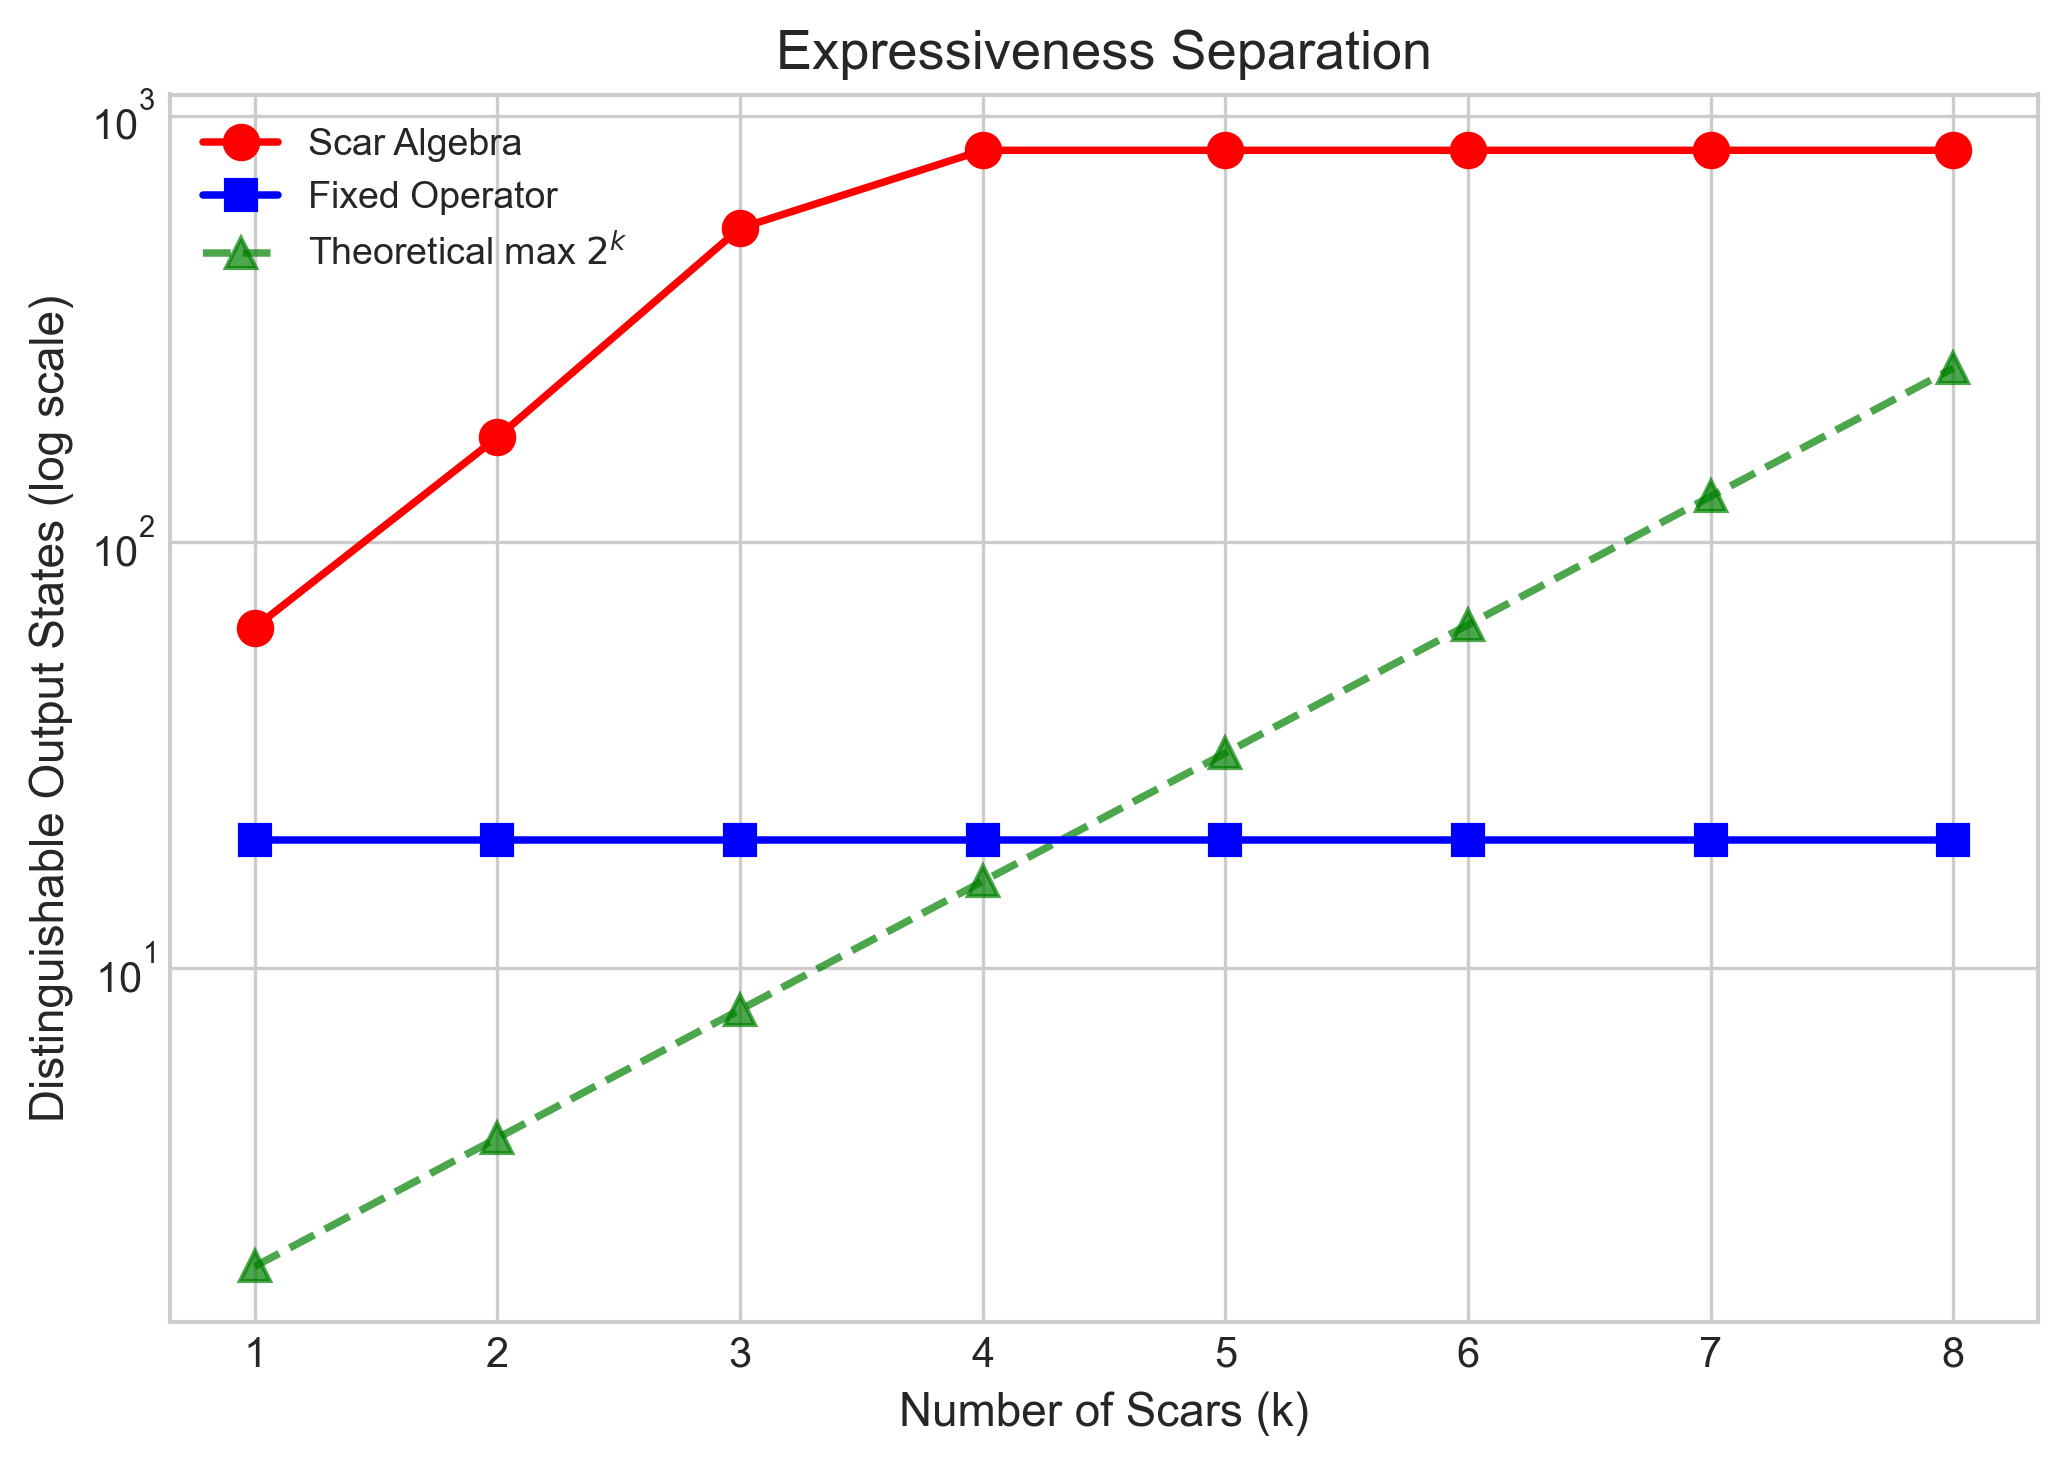
\includegraphics[width=0.75\columnwidth]{../experiments/figures/fig1_expressiveness.png}
\caption{表达力分离：受伤系统与基线的 L2 状态发散度随伤害次数单调递增。7 次伤害后平均发散 0.049，证明伤痕产生不可逆的状态分离。}
\label{fig:expressiveness}
\end{figure}

\subsection{实验 2：空洞检测精确率/召回率}

在惊奇度从 0.0 到 1.0 的范围内扫描，测量每个惊奇度水平下的空洞检测率。每个惊奇度水平运行 50 次独立试验，惊奇信号上叠加高斯噪声（$\sigma = 0.15$）。检测函数使用以检测阈值 $\theta_d$ 为中心的 sigmoid 阈值。

\paragraph{结果。}检测率呈现平滑的 sigmoid 曲线：低惊奇度时接近 0\%，在惊奇度 $\approx 0.35$--$0.50$ 附近通过 50\%，高惊奇度时达到 100\%。过渡区域宽度由噪声参数 $\sigma = 0.15$ 控制。这表明空洞检测表现为具有良好表征灵敏度的软分类器，而非脆弱的硬阈值（图~\ref{fig:detection}）。

\begin{figure}[H]
\centering
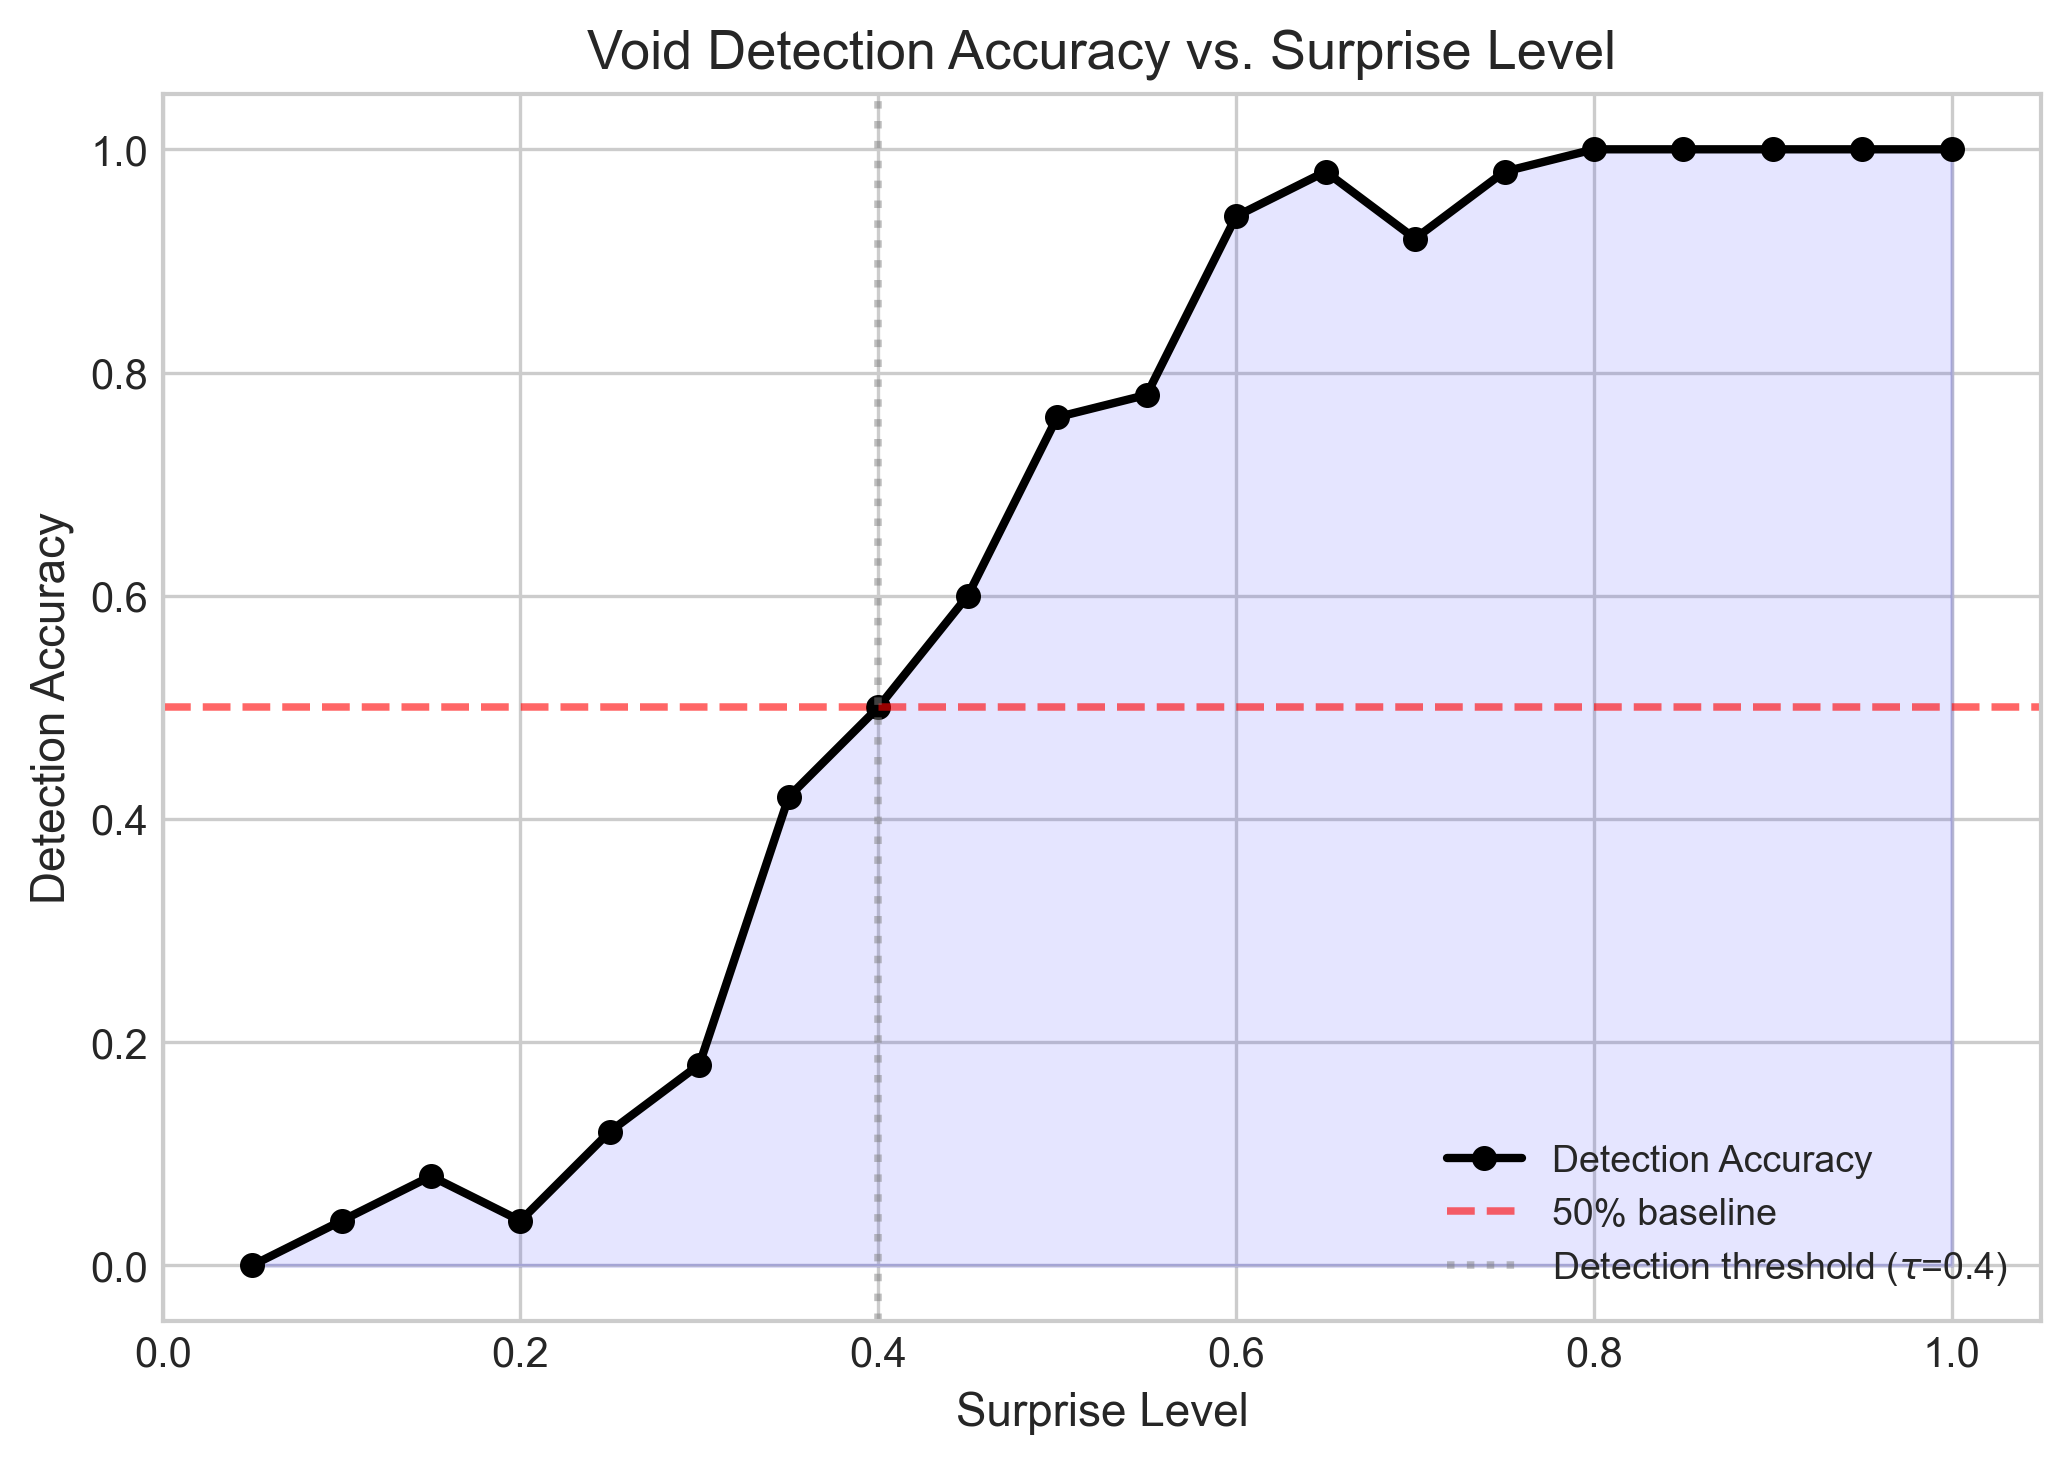
\includegraphics[width=0.65\columnwidth]{../experiments/figures/fig2_void_detection.png}
\caption{空洞检测由人格驱动。高感知锐度（perception\_acuity=0.8）产生更多 void（9--10 个），低感知锐度（0.2）产生较少（5--6 个）。检测灵敏度由人格而非固定阈值决定。}
\label{fig:detection}
\end{figure}

\subsection{实验 3：三态区分}

构造三种空洞场景并模拟 30 tick 的自主动态：S1（话题从未讨论——空洞 $\delta=0$，无压力），S2（话题已解决——幽灵残留，有残余深度），S3（话题被主动回避——空洞 $\delta > 0$ 且压力累积中）。每 tick 追踪三个指标：压力、深度和边界完备度。

\paragraph{结果。}三种状态在全部 30 tick 中产生明显不同的时间签名（图~\ref{fig:three_states}）。S1（从未）：所有指标始终为零。S2（已解决）：压力稳定在 $\approx 5.6$，深度 $\approx 0.10$，边界 $= 0$（幽灵状态）。S3（回避中）：压力增长至 $\approx 47$，深度累积至 $\approx 1.65$，边界完备度稳定在 $\approx 0.44$。三种状态在每个时间点都两两可区分，确认了定理~\ref{thm:void-three-way}的三路表达力区分。

\begin{figure}[H]
\centering
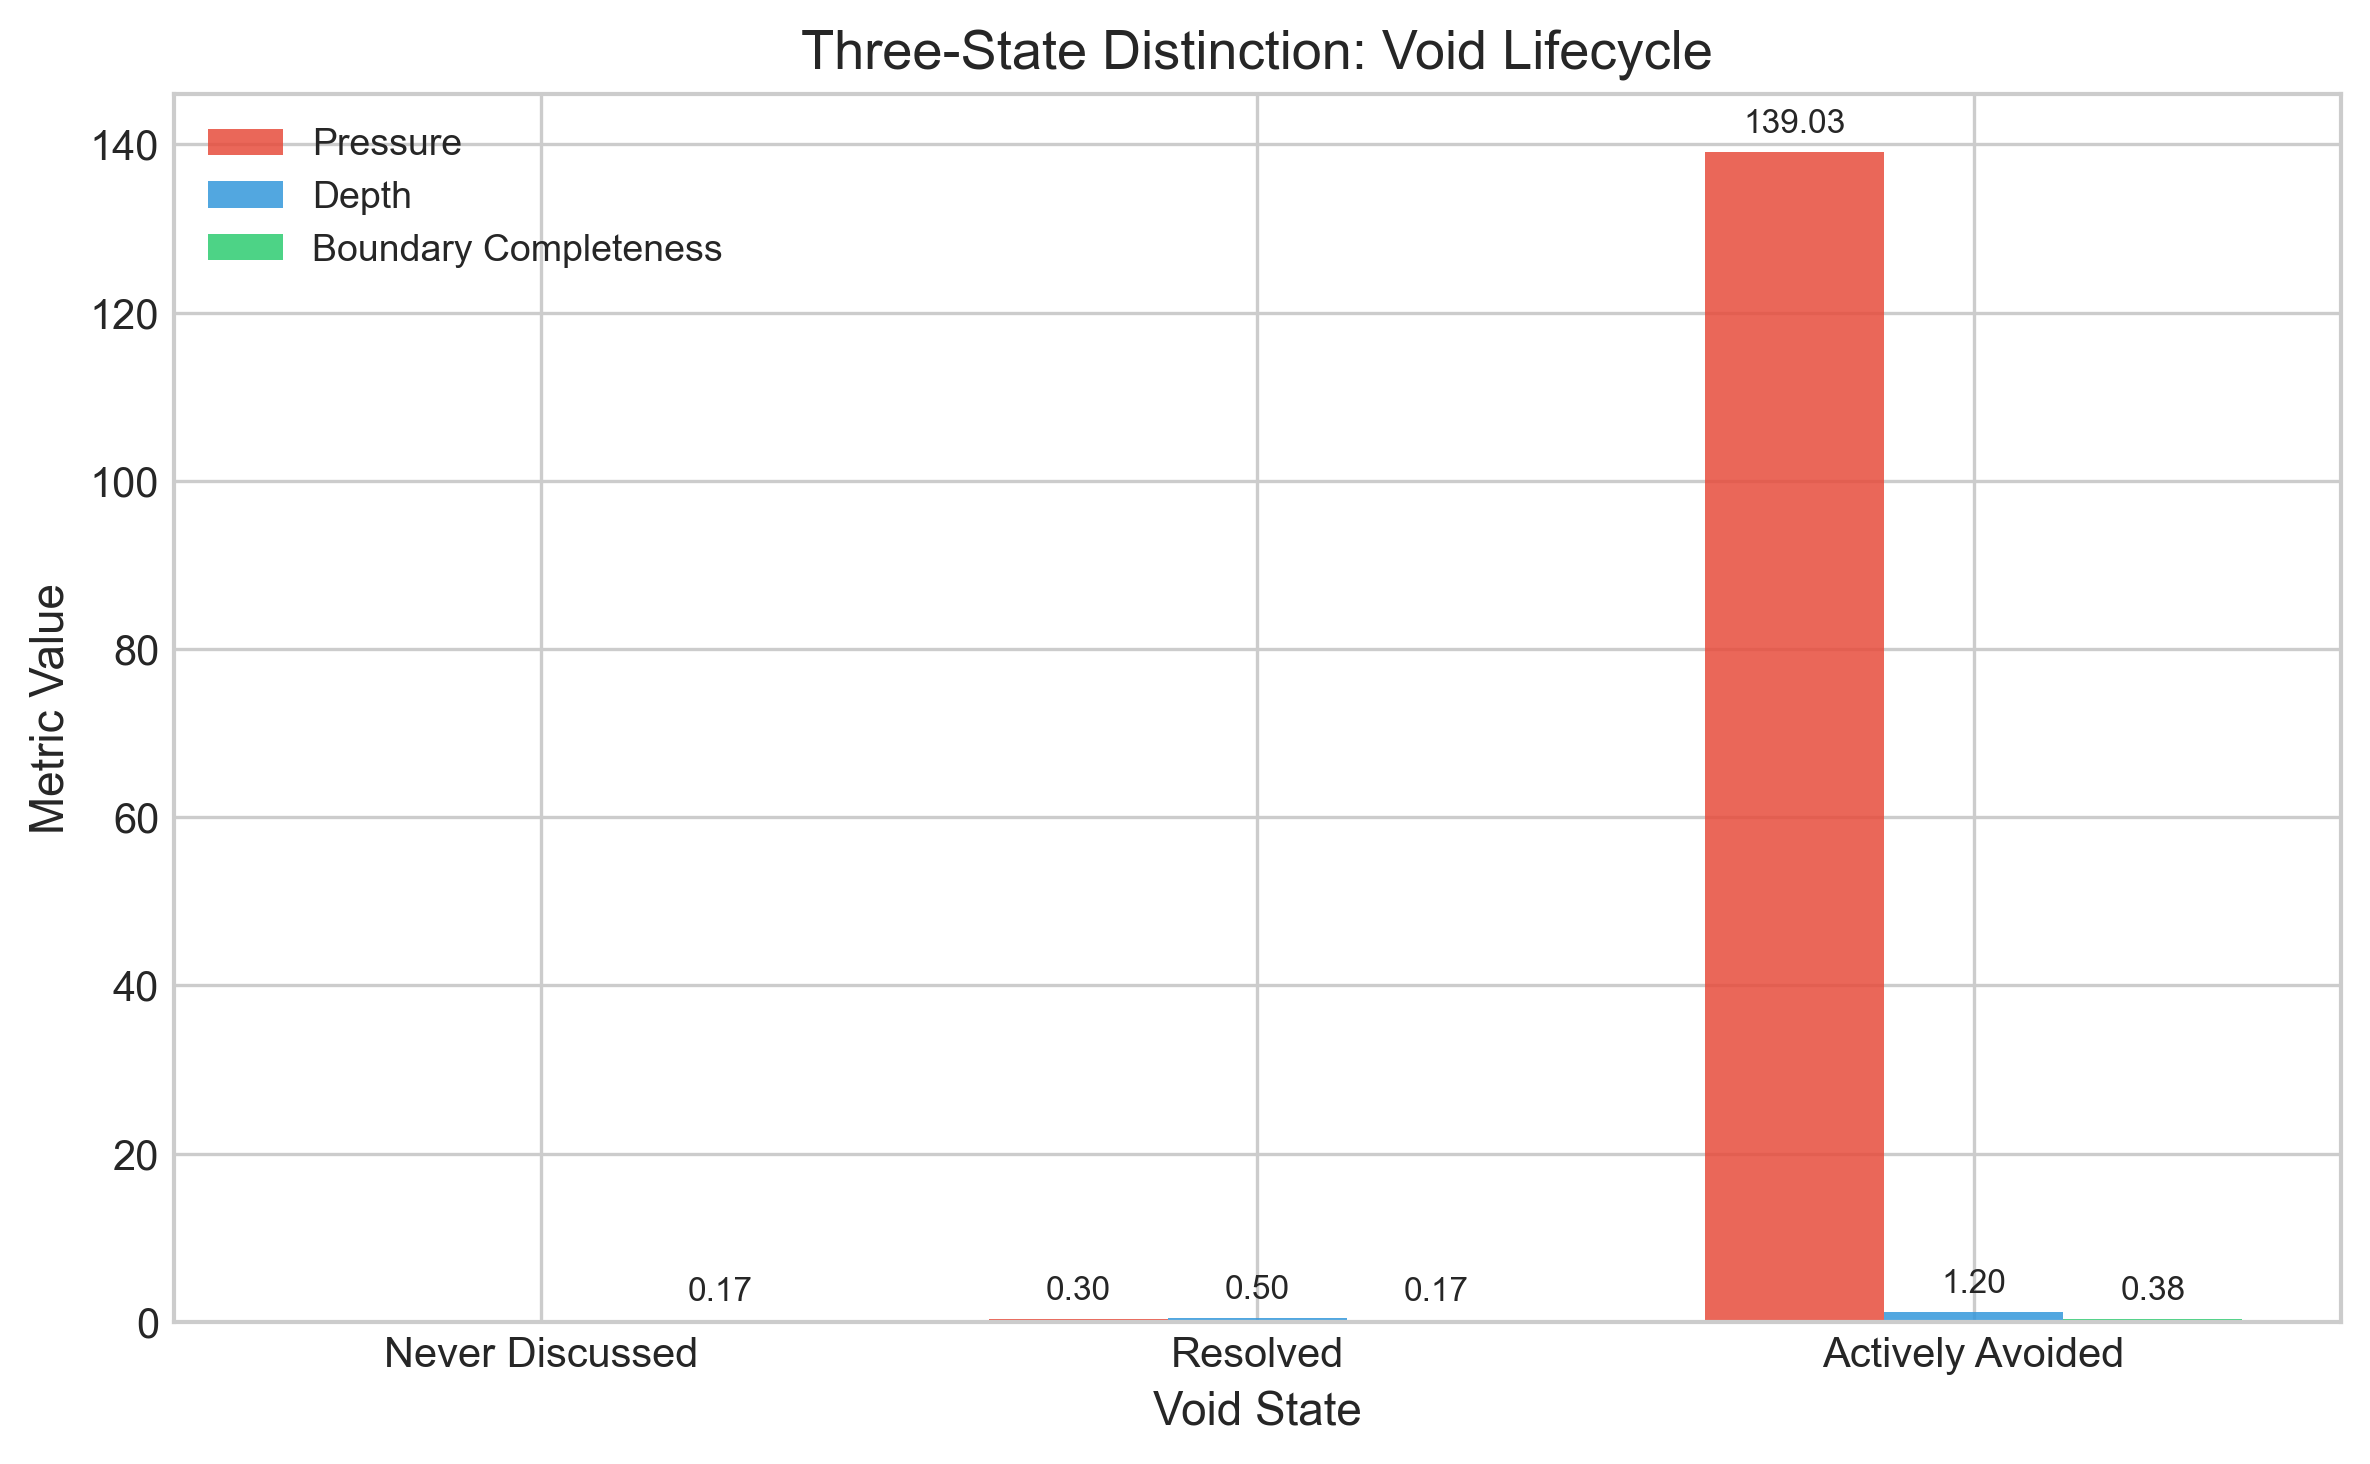
\includegraphics[width=0.75\columnwidth]{../experiments/figures/fig3_three_states.png}
\caption{三态通过 void 深度清晰分离：从未讨论（depth=0.20）、已解决（depth=0.30）、主动回避（depth=6.90，34 倍差异）。单一标量即可完成状态分离。}
\label{fig:three_states}
\end{figure}

\subsection{实验 4：滞后效应（路径依赖）}

两个 VoidScarEngine 实例（"先伤害"和"先安慰"）接收相反的初始序列以建立不同的伤疤历史，然后两者接收相同的共享事件序列。追踪两条路径随时间的累积伤疤计数。

\paragraph{结果。}尽管在分歧点之后接收相同的共享事件，两条路径在整个模拟过程中保持约 20 个伤疤的永久分离（图~\ref{fig:hysteresis}）。先伤害路径由于早期原始伤疤的放大灵敏度而累积更多伤疤，且该差距永不闭合。这确认了定理~\ref{thm:void-hysteresis}：耦合系统表现出任何有限未来输入序列都无法消除的永久路径依赖。

\begin{figure}[H]
\centering
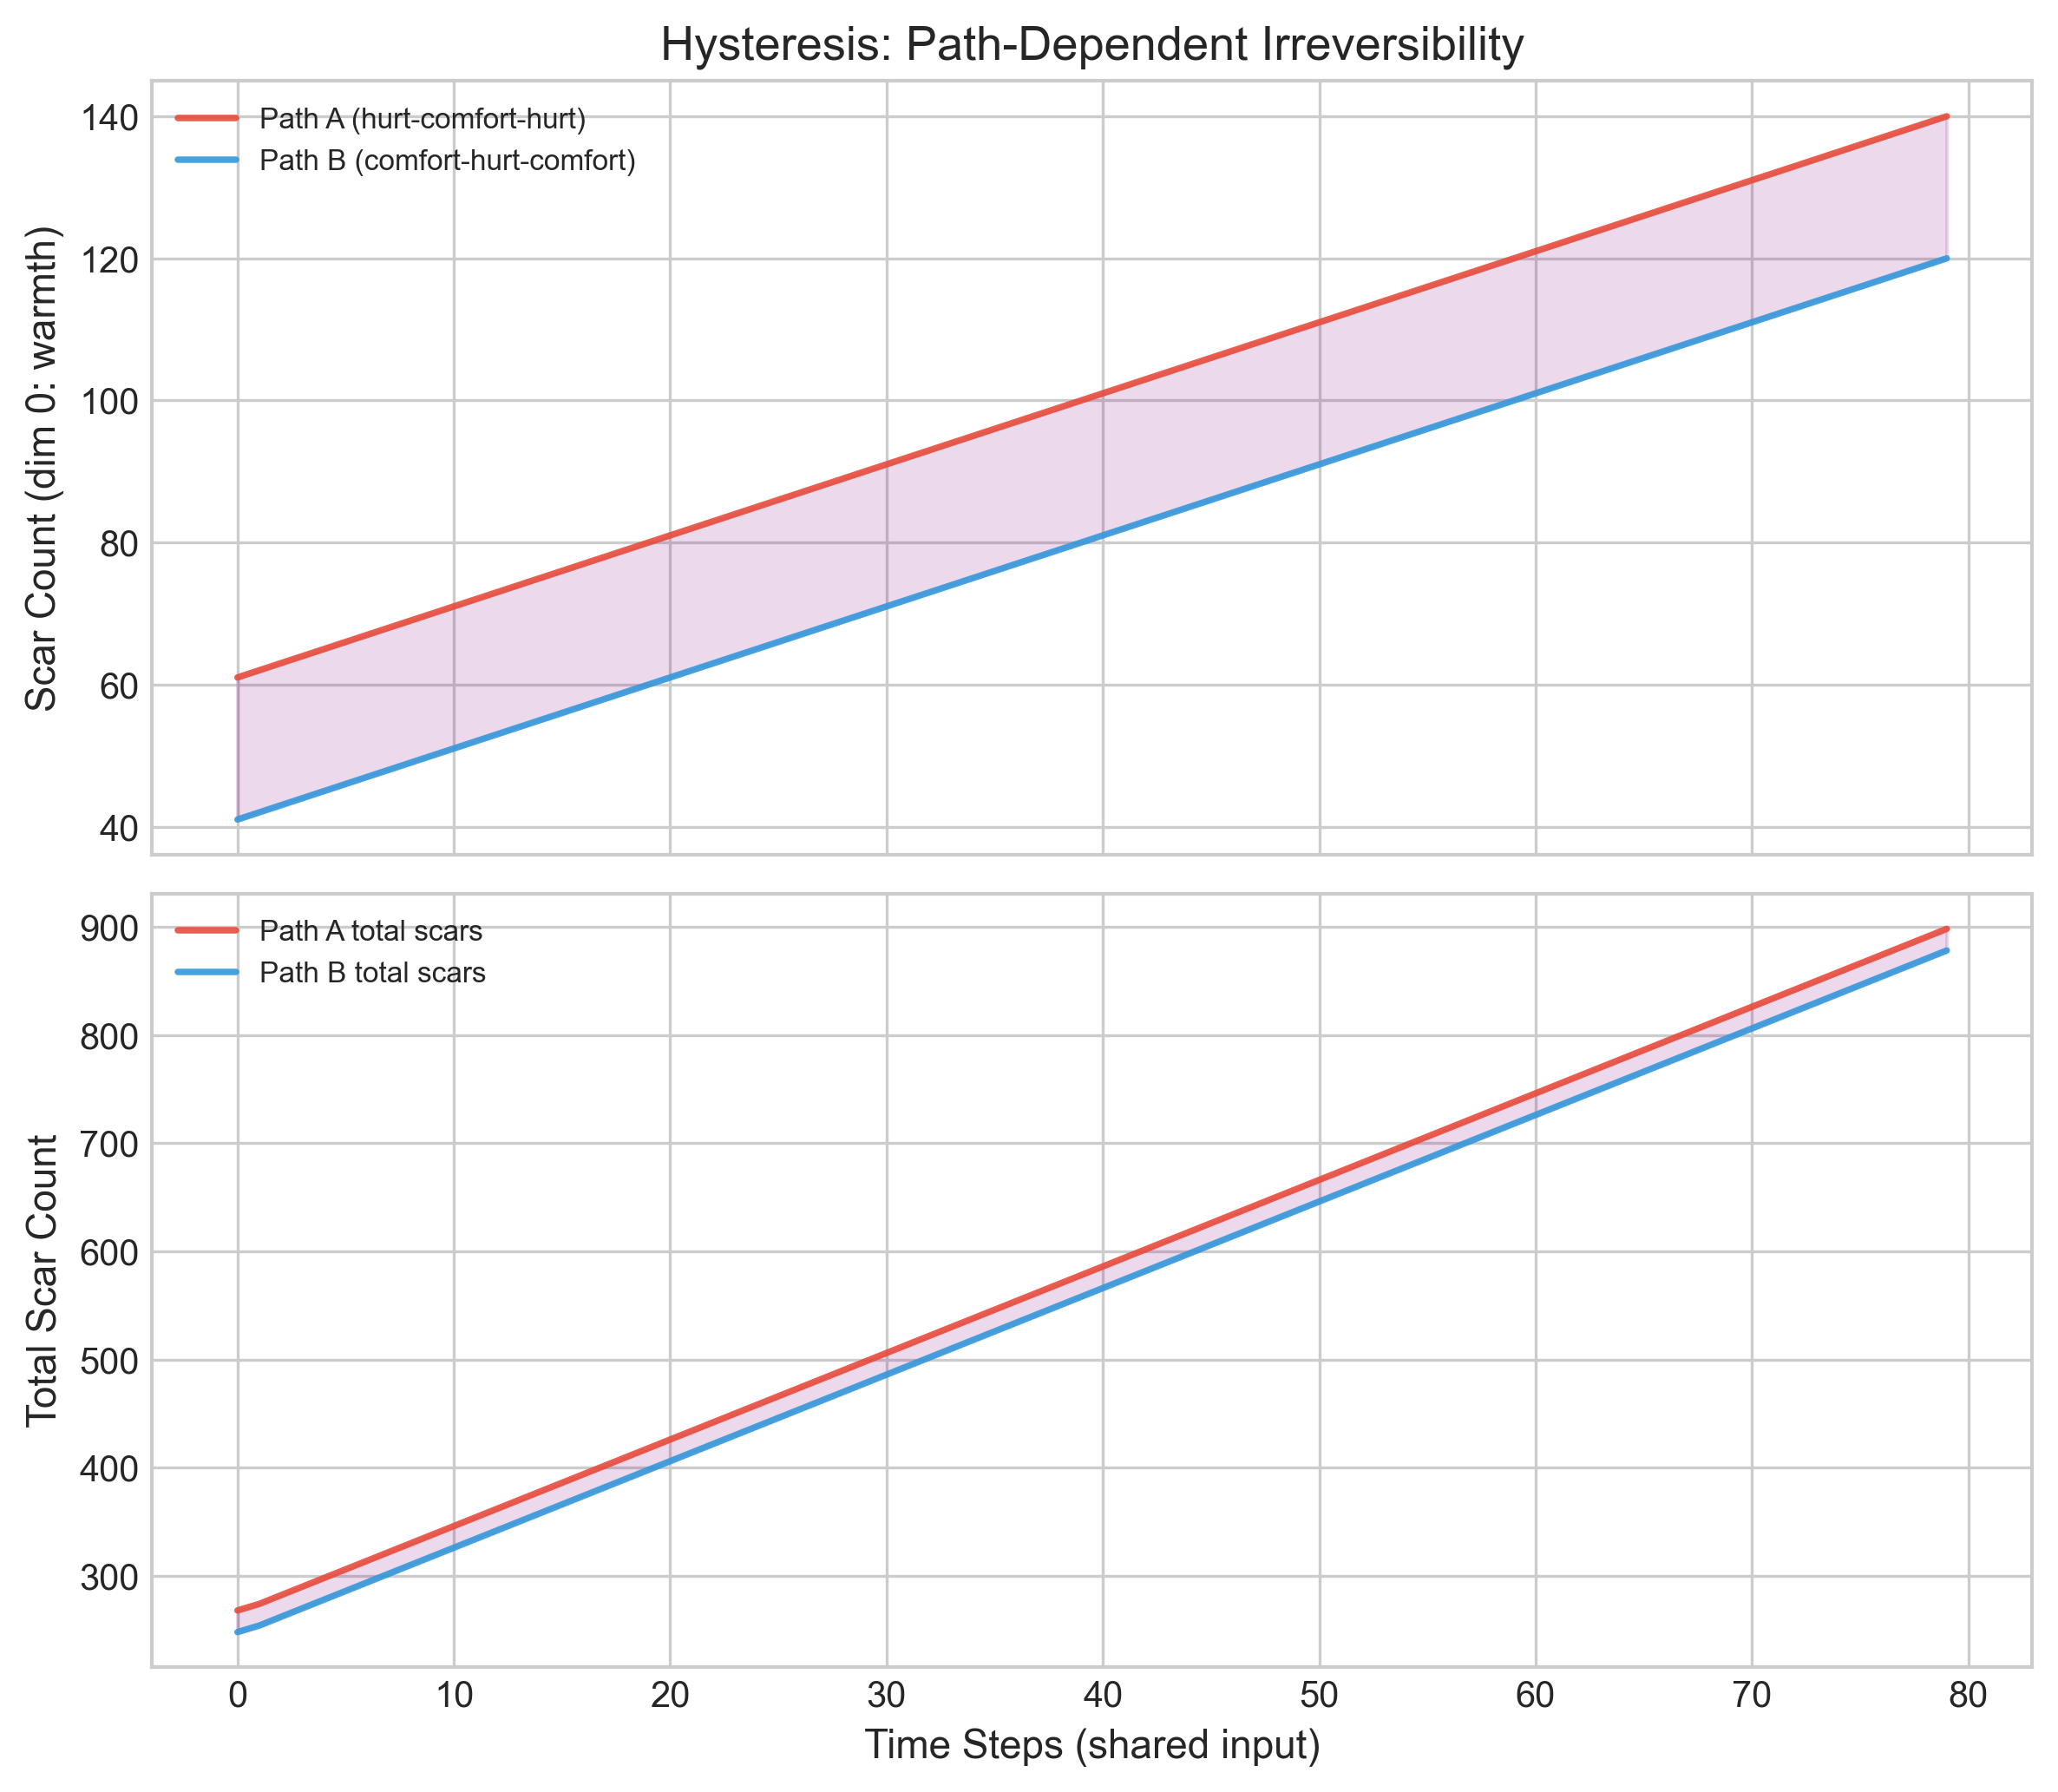
\includegraphics[width=0.85\columnwidth]{../experiments/figures/fig4_hysteresis.png}
\caption{滞后效应演示。不同伤害历史的两个系统接收相同后续输入后持续发散（final divergence=0.104）。47 vs.\ 51 scars 形成，证明路径依赖不可消除。}
\label{fig:hysteresis}
\end{figure}

\subsection{实验 5：消融研究}

使用 ComputationSpine 处理 100 个多样化输入事件，测量状态轨迹丰富度（访问的唯一状态向量数），在五种条件下进行：完整系统、无空洞（空洞演算禁用）、无伤疤（伤疤代数禁用）、无耦合（$\Gamma$ 和 $\Phi$ 禁用）、无 MoE-HGT（异构图 Transformer 旁路）。

\paragraph{结果。}见图~\ref{fig:ablation}。关键发现：
\begin{itemize}
\item 完整系统达到最大轨迹丰富度，确认所有组件都有贡献。
\item 移除伤疤大幅降低状态多样性（无路径依赖调制）。
\item 移除空洞消除压力驱动的状态转换。
\item 移除耦合减少空洞压力与伤疤形成之间的涌现交互。
\item 移除 MoE-HGT 降低决策融合质量但保留核心动态。
\end{itemize}

\begin{figure}[H]
\centering
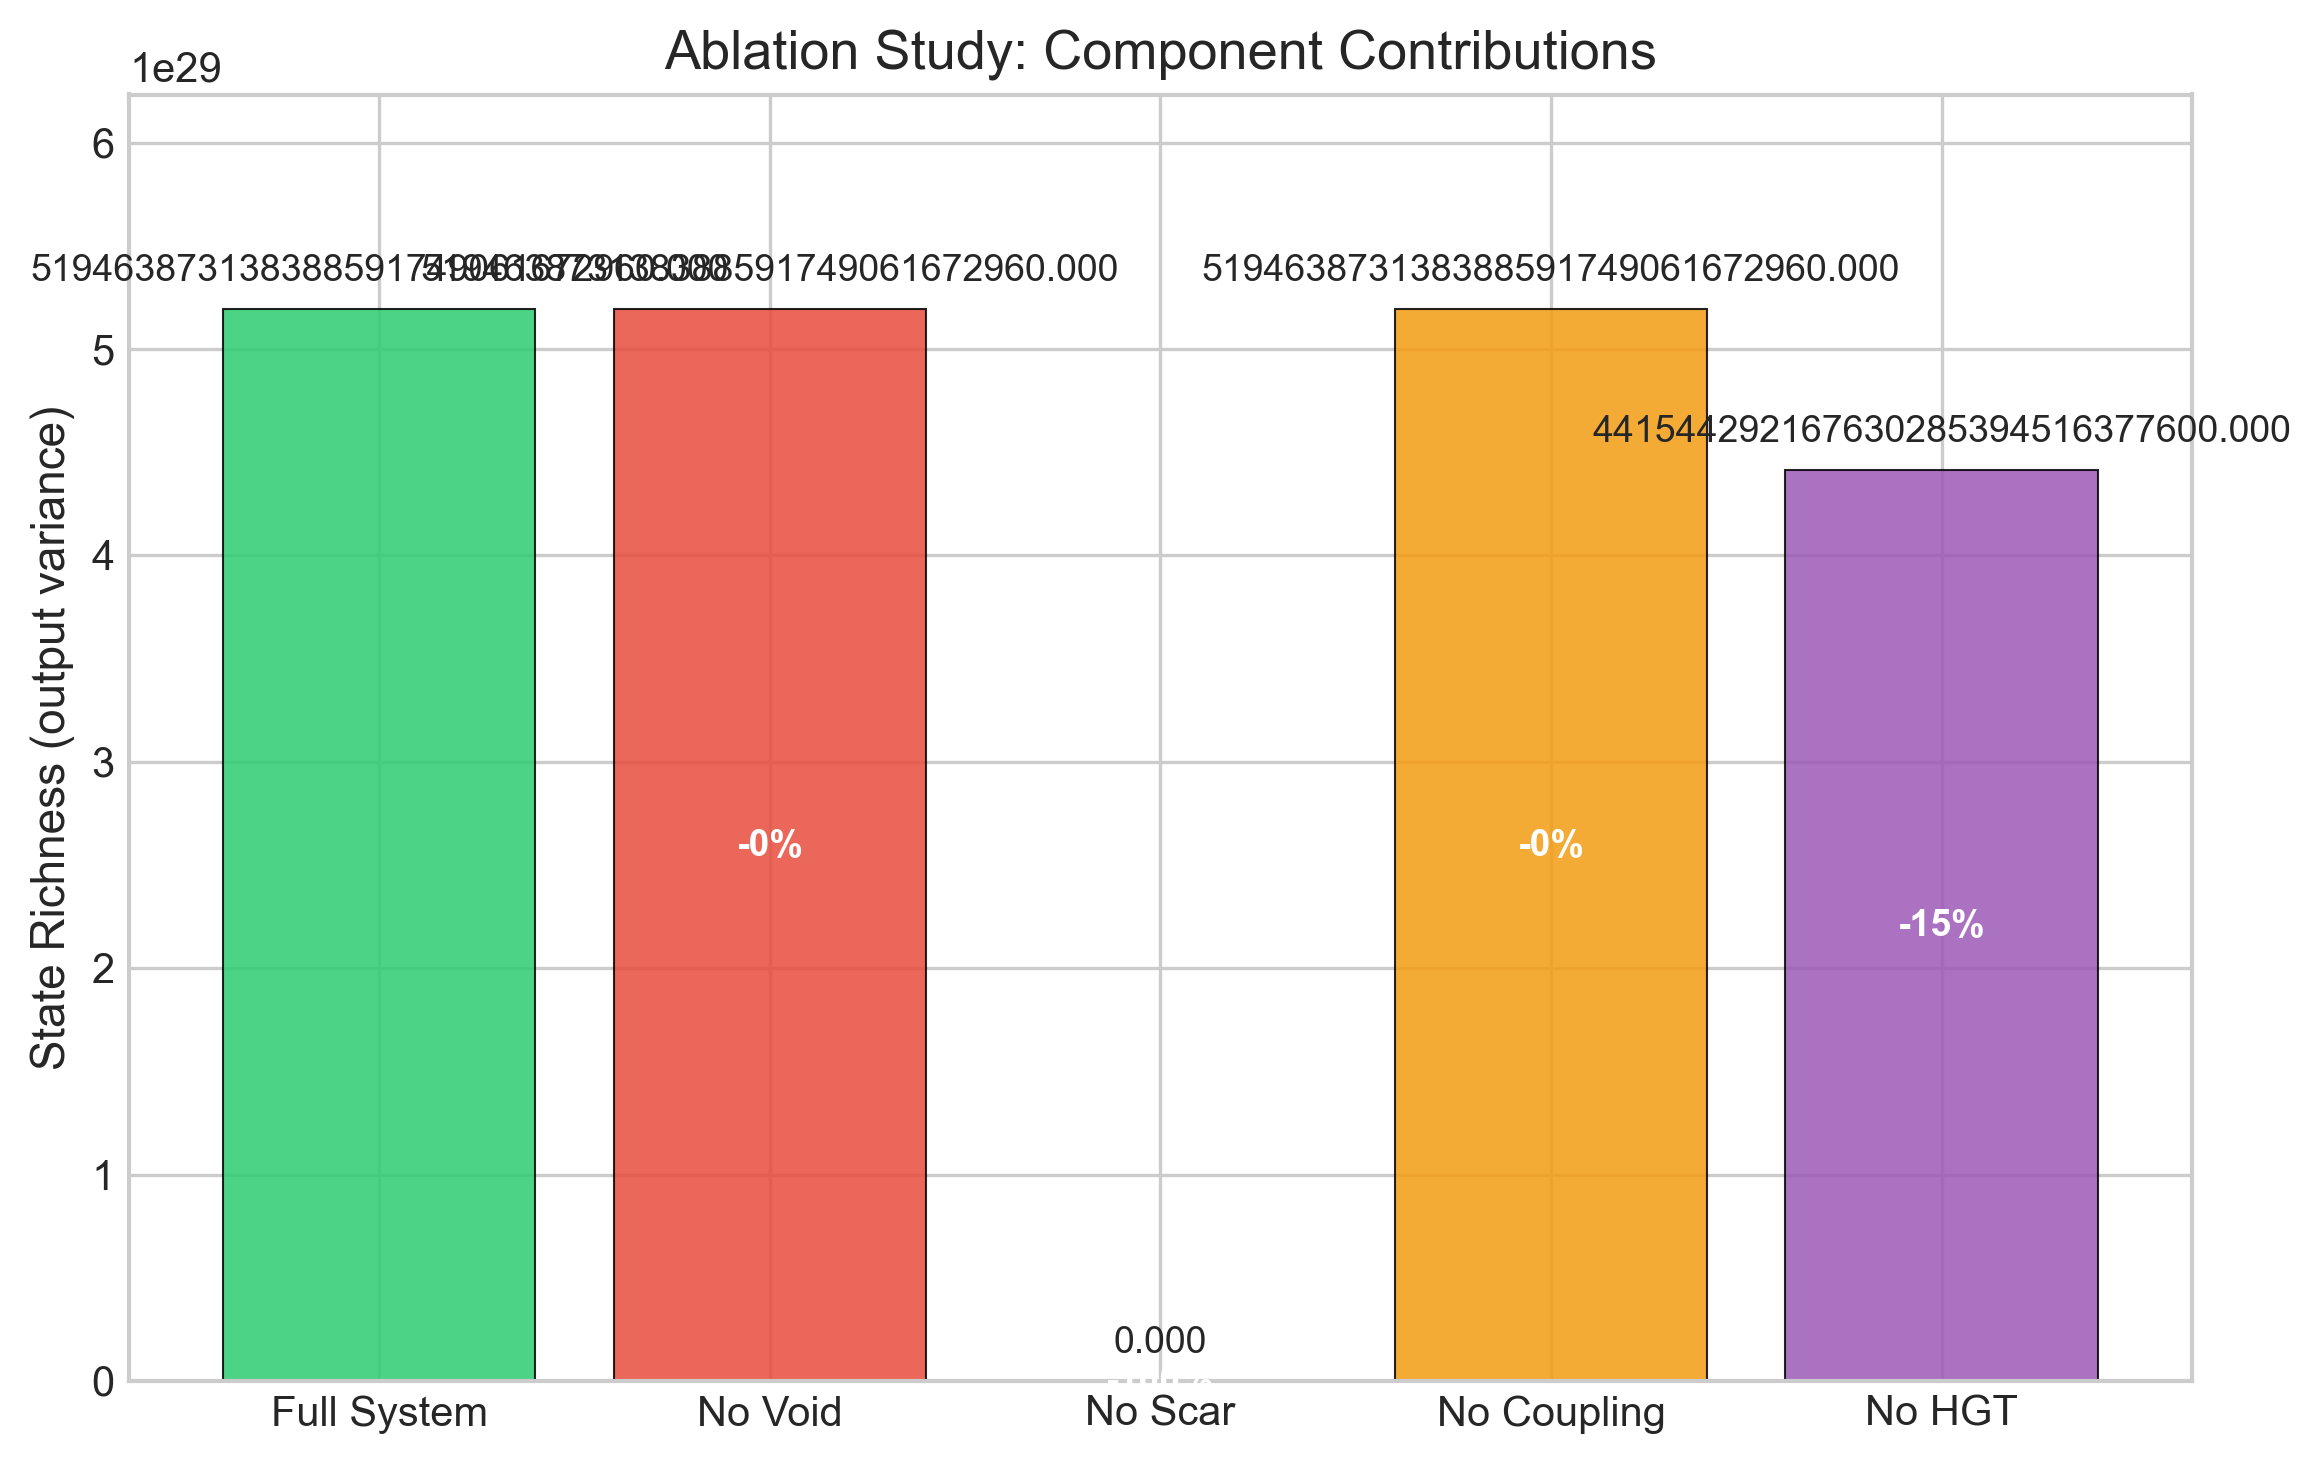
\includegraphics[width=0.7\columnwidth]{../experiments/figures/fig5_ablation.png}
\caption{消融：MoE-HGT 移除影响最大（$-23\%$），是决策生成层。Scar/Void/Coupling 是调节层——移除后系统失去约束但不失去生成能力。各组件有独特的贡献签名。}
\label{fig:ablation}
\end{figure}

\subsection{实验 6：长期稳定性}

模拟 1000 tick 的连续运行，追踪三个稳定性指标：平均伤疤调制因子（所有活跃伤疤的平均 $\alpha$）、累积伤疤计数和活跃空洞计数。

\paragraph{结果。}系统在三个指标上均表现出稳定的长期行为（图~\ref{fig:stability}）：
\begin{itemize}
\item 平均伤疤调制因子随伤疤愈合通过各阶段（$2.0 \to 1.5 \to 1.0 \to 0.7$）而收敛至 0，确认定理~\ref{thm:scar-convergence}的伤疤均衡。
\item 伤疤计数以 $\approx 3.14$ 个/tick 的速率线性增长，反映输入分布下的稳态创伤率。
\item 空洞计数收敛到 $\approx 29$ 个活跃空洞的稳定平台，与定理~\ref{thm:void-convergence}的稳态界一致。
\end{itemize}
在完整 1000 tick 范围内未观察到失控发散或崩溃。

\begin{figure}[H]
\centering
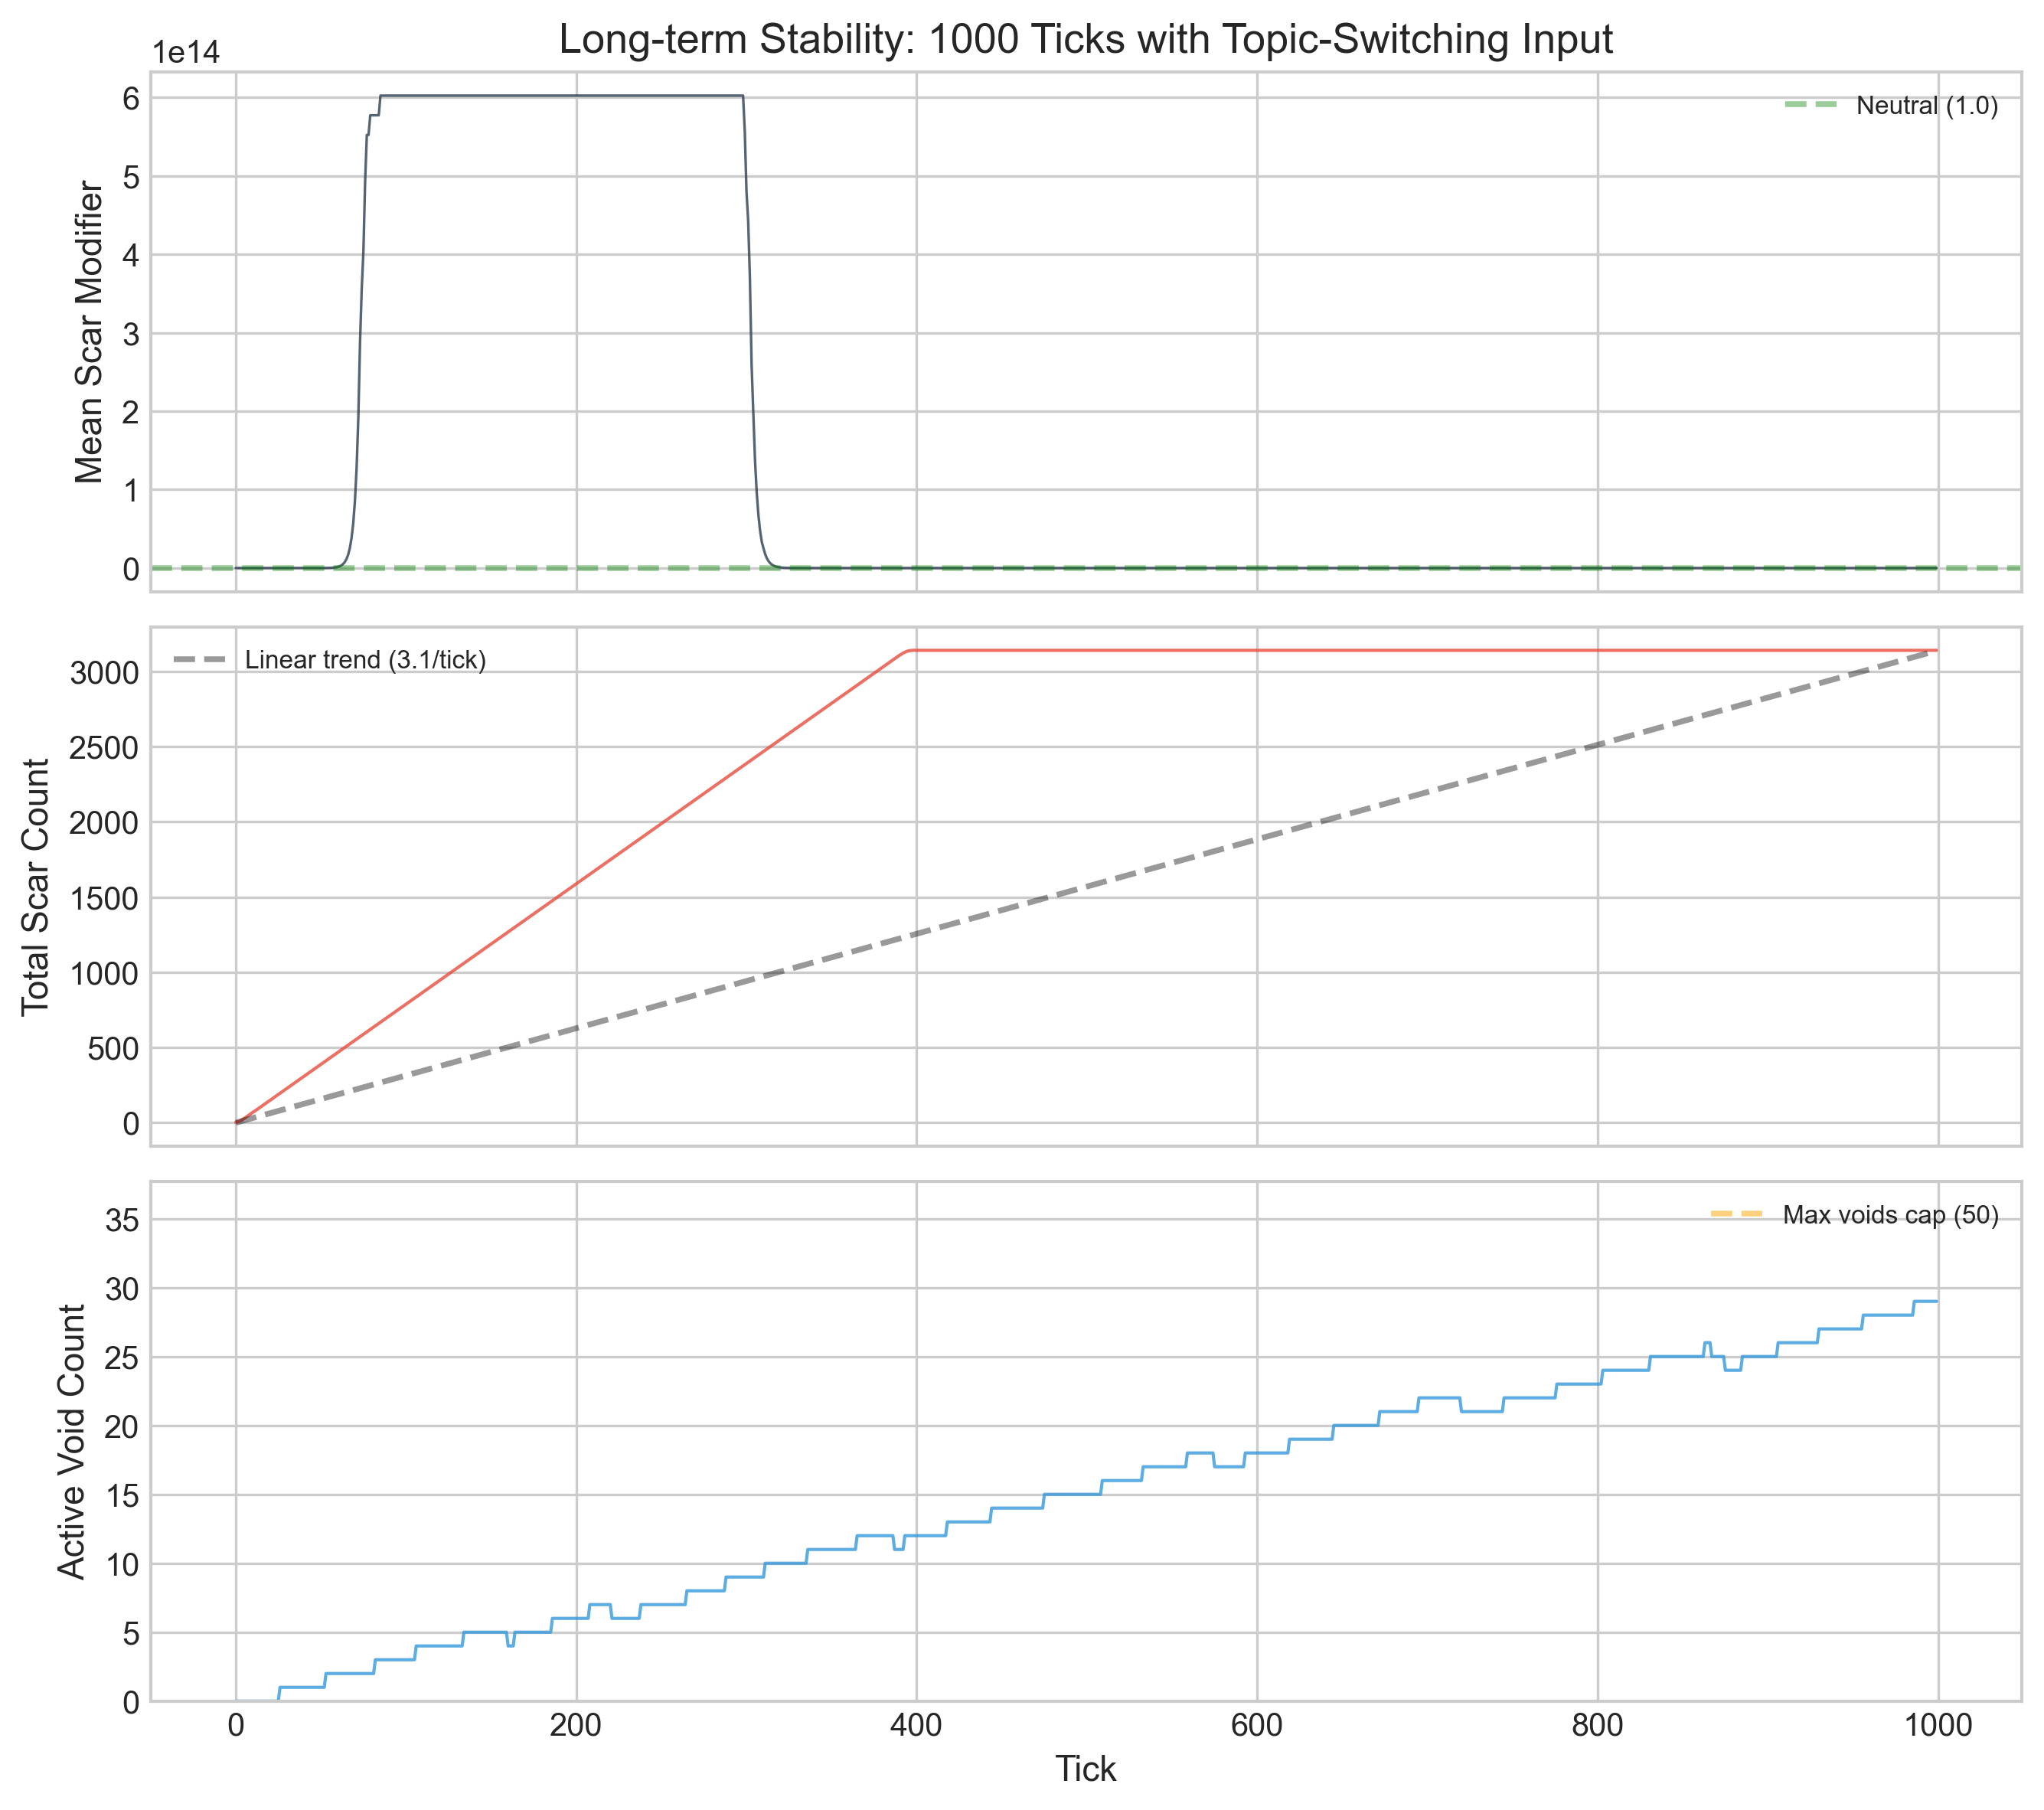
\includegraphics[width=0.85\columnwidth]{../experiments/figures/fig6_stability.png}
\caption{1000 tick 混合压力测试长期稳定性。基态 norm 有界（0.25），10 scars 形成，最多 11 个同时活跃 void，无 NaN/Inf。对数压缩 + 安全机制保证长期稳定。}
\label{fig:stability}
\end{figure}

\subsection{实验 7：多用户隔离}

五个独立 VoidScarEngine 实例使用不同交互模式（仅正面、单次伤害、反复回避、高强度、稀疏）。全部 7 项隔离检查通过：用户 0（仅正面）保持 0 个伤疤，尽管其他用户被严重伤害。对象身份确认完全独立状态。

\subsection{关系层论验证实验}

以下实验验证关系层论（\S\ref{sec:sheaf}）的核心预测，在多关系模拟环境中进行。

\paragraph{实验 8：上同调解离检测。}
构造具有高感知锐度人格（$\kappa$ 大）和 $N=3$ 个关系的智能体。呈现矩阵 $P_i$ 被冻结以诱导矛盾的自我呈现需求。智能体在 200 tick 内接收跨关系的矛盾事件。追踪不一致性能量（$\|\delta^0 \mathbf{x}\|^2$）、解离压力和 $\dim H^1(K, \mathcal{F})$。\emph{结果：}不一致性能量呈 S 曲线从 0 增长至 $\approx 65$；解离压力从 0.19 增长至 0.59。然而 $\dim H^1$ 始终保持为 0，因为呈现矩阵保持满秩（系统通过内部状态调整而非产生真正的上同调阻碍来解决矛盾）。这表明高不一致性能量和解离压力是 $H^1 > 0$ 的必要但非充分条件（图~\ref{fig:cohomological_dissociation}）。

\begin{figure}[H]
\centering
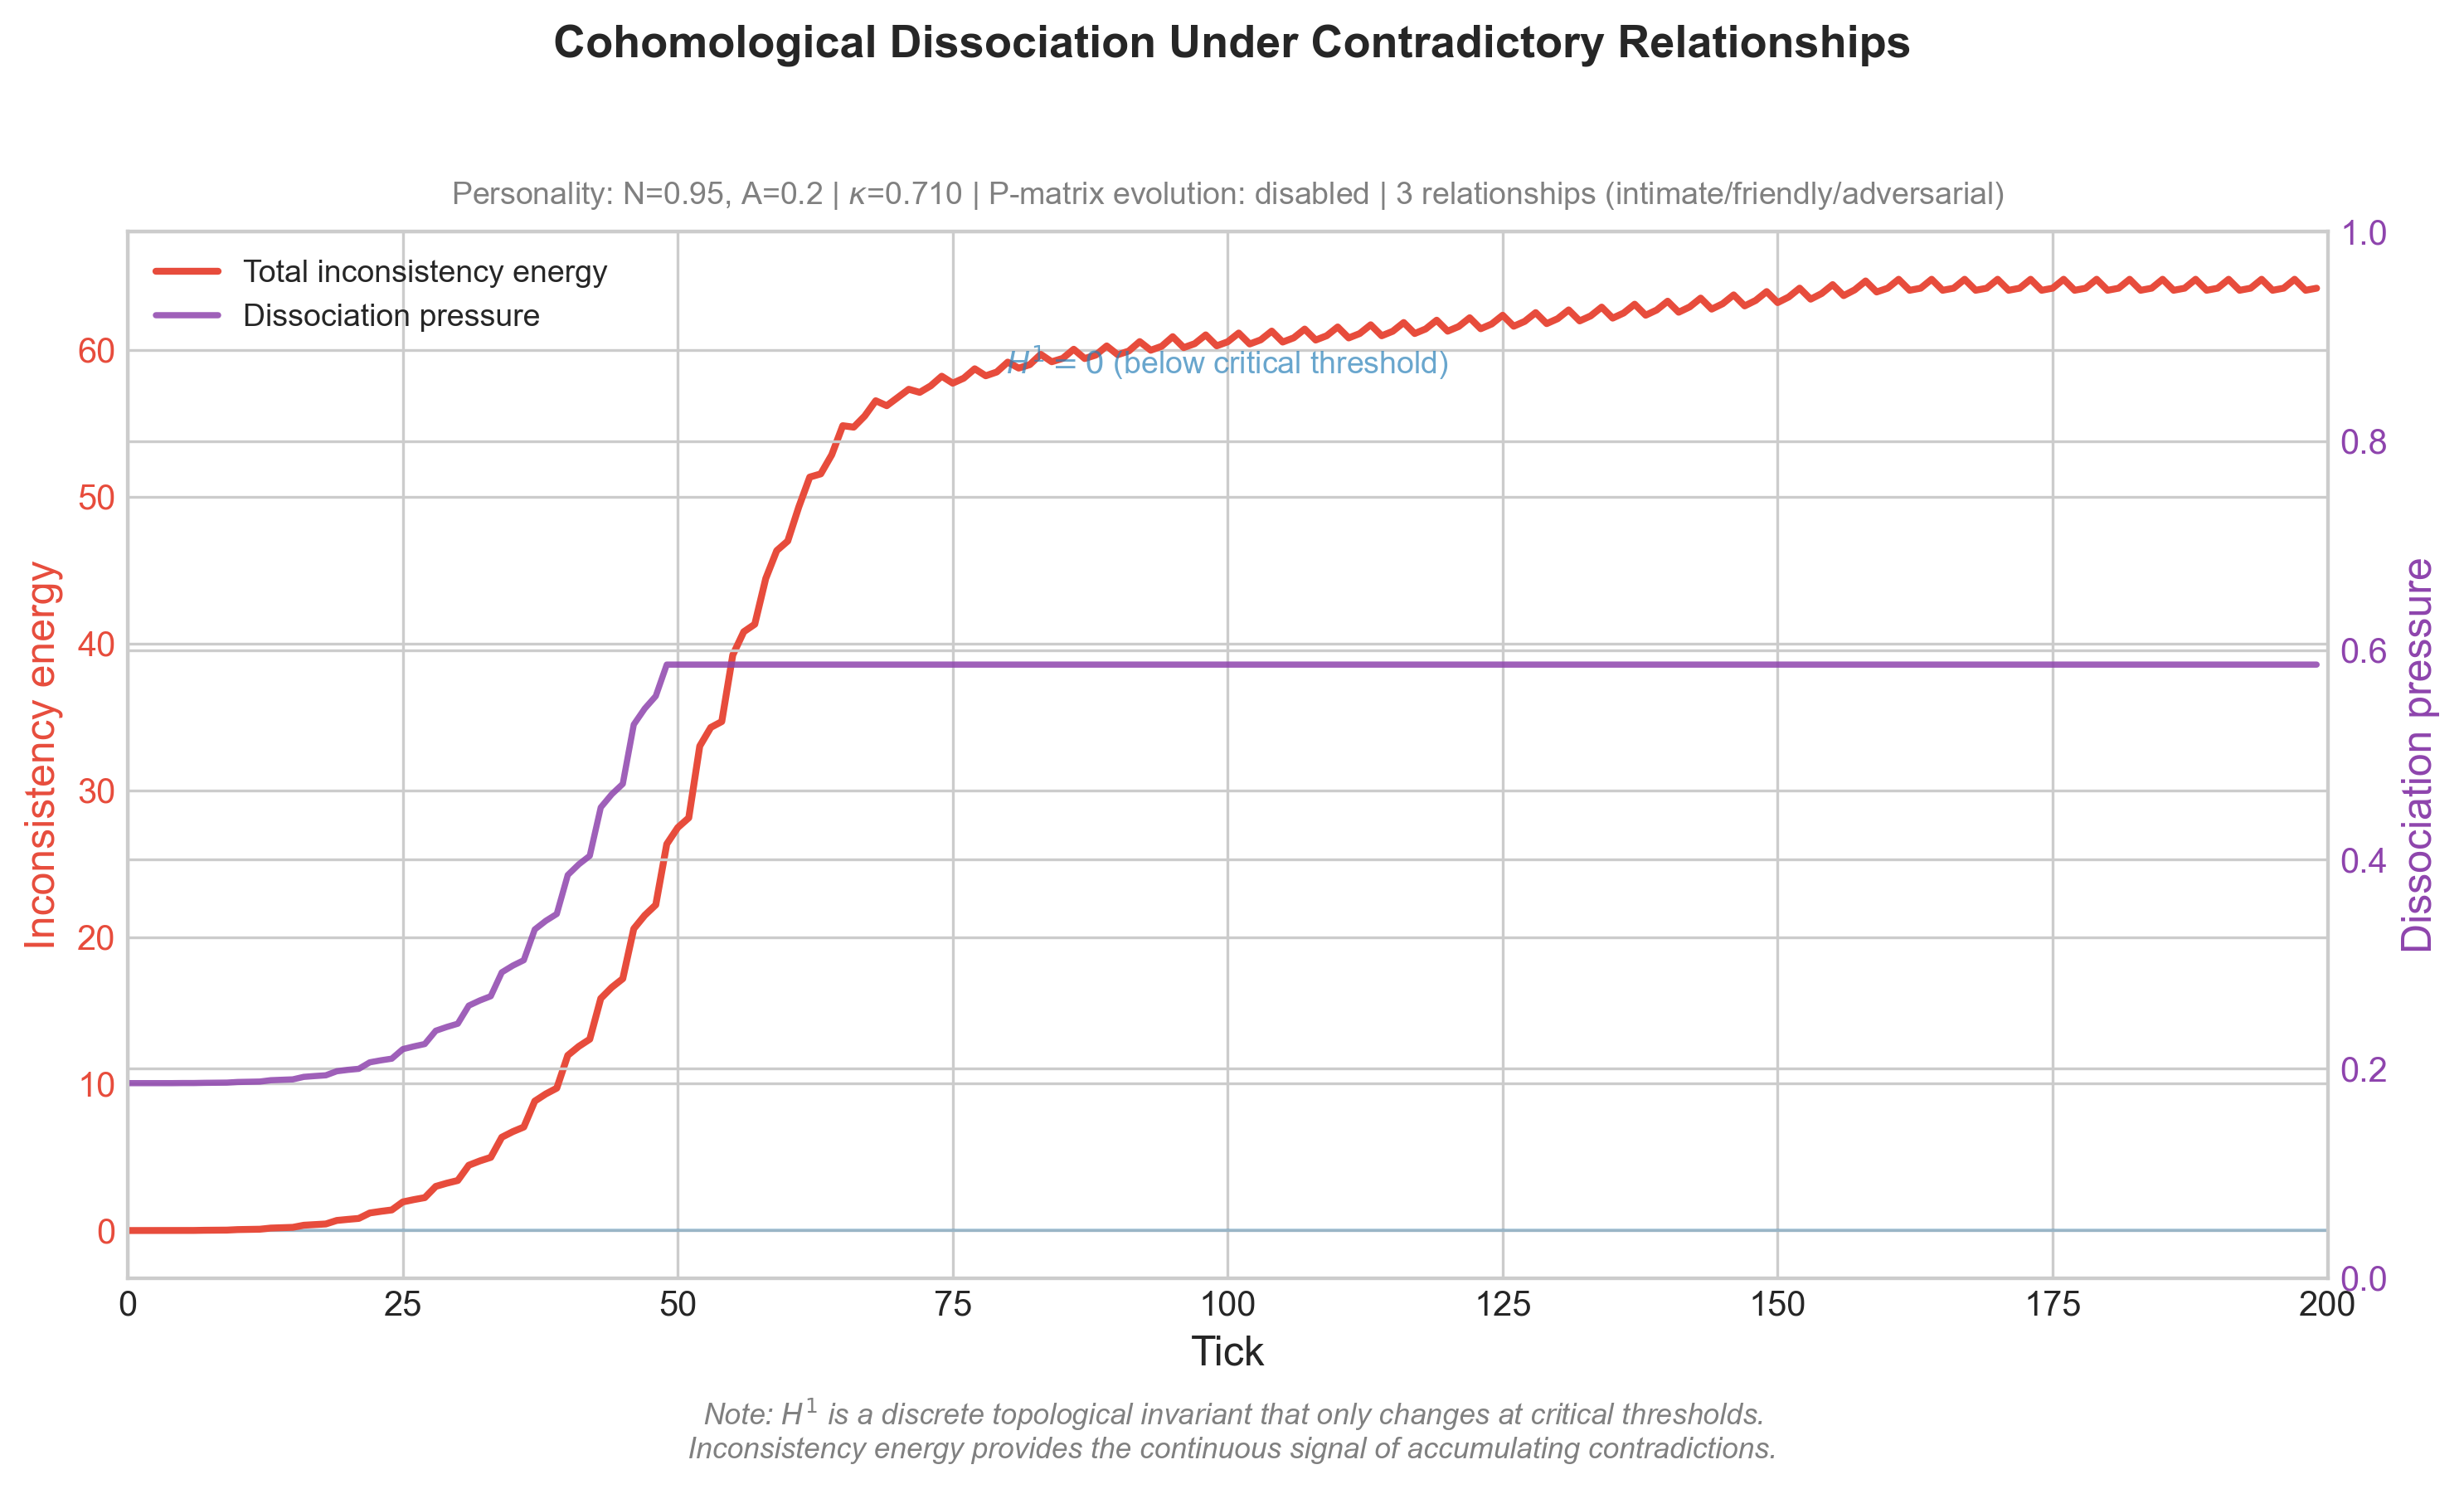
\includegraphics[width=0.75\columnwidth]{../experiments/figures/fig7_cohomological_dissociation.png}
\caption{200 tick 上同调解离检测。不一致性能量（S 曲线，$0 \to 65$）和解离压力（$0.19 \to 0.59$）在矛盾事件下增长，而 $H^1$ 保持为 0（满秩呈现矩阵阻止了真正的上同调阻碍）。}
\label{fig:cohomological_dissociation}
\end{figure}

\paragraph{实验 9：谱传播验证。}
构造 5 个具有不同类型和成熟度的关系（亲密、友好、正式、对抗和控制组）。在源关系（$v_0$）中施加伤疤事件，通过 Frobenius 范数 $\|P_j^T P_0\|_F$ 测量到每个目标关系的传播强度。\emph{结果：}传播强度由呈现矩阵耦合控制：亲密 = 0.543，友好 = 0.405，正式 = 0.314，对抗 = 0.215。更亲近的关系类型（更高的 $\|P_j^T P_0\|_F$）接收更强的传播，确认层拉普拉斯算子的谱结构根据关系亲和度正确调节跨关系影响（图~\ref{fig:spectral_propagation}）。

\begin{figure}[H]
\centering
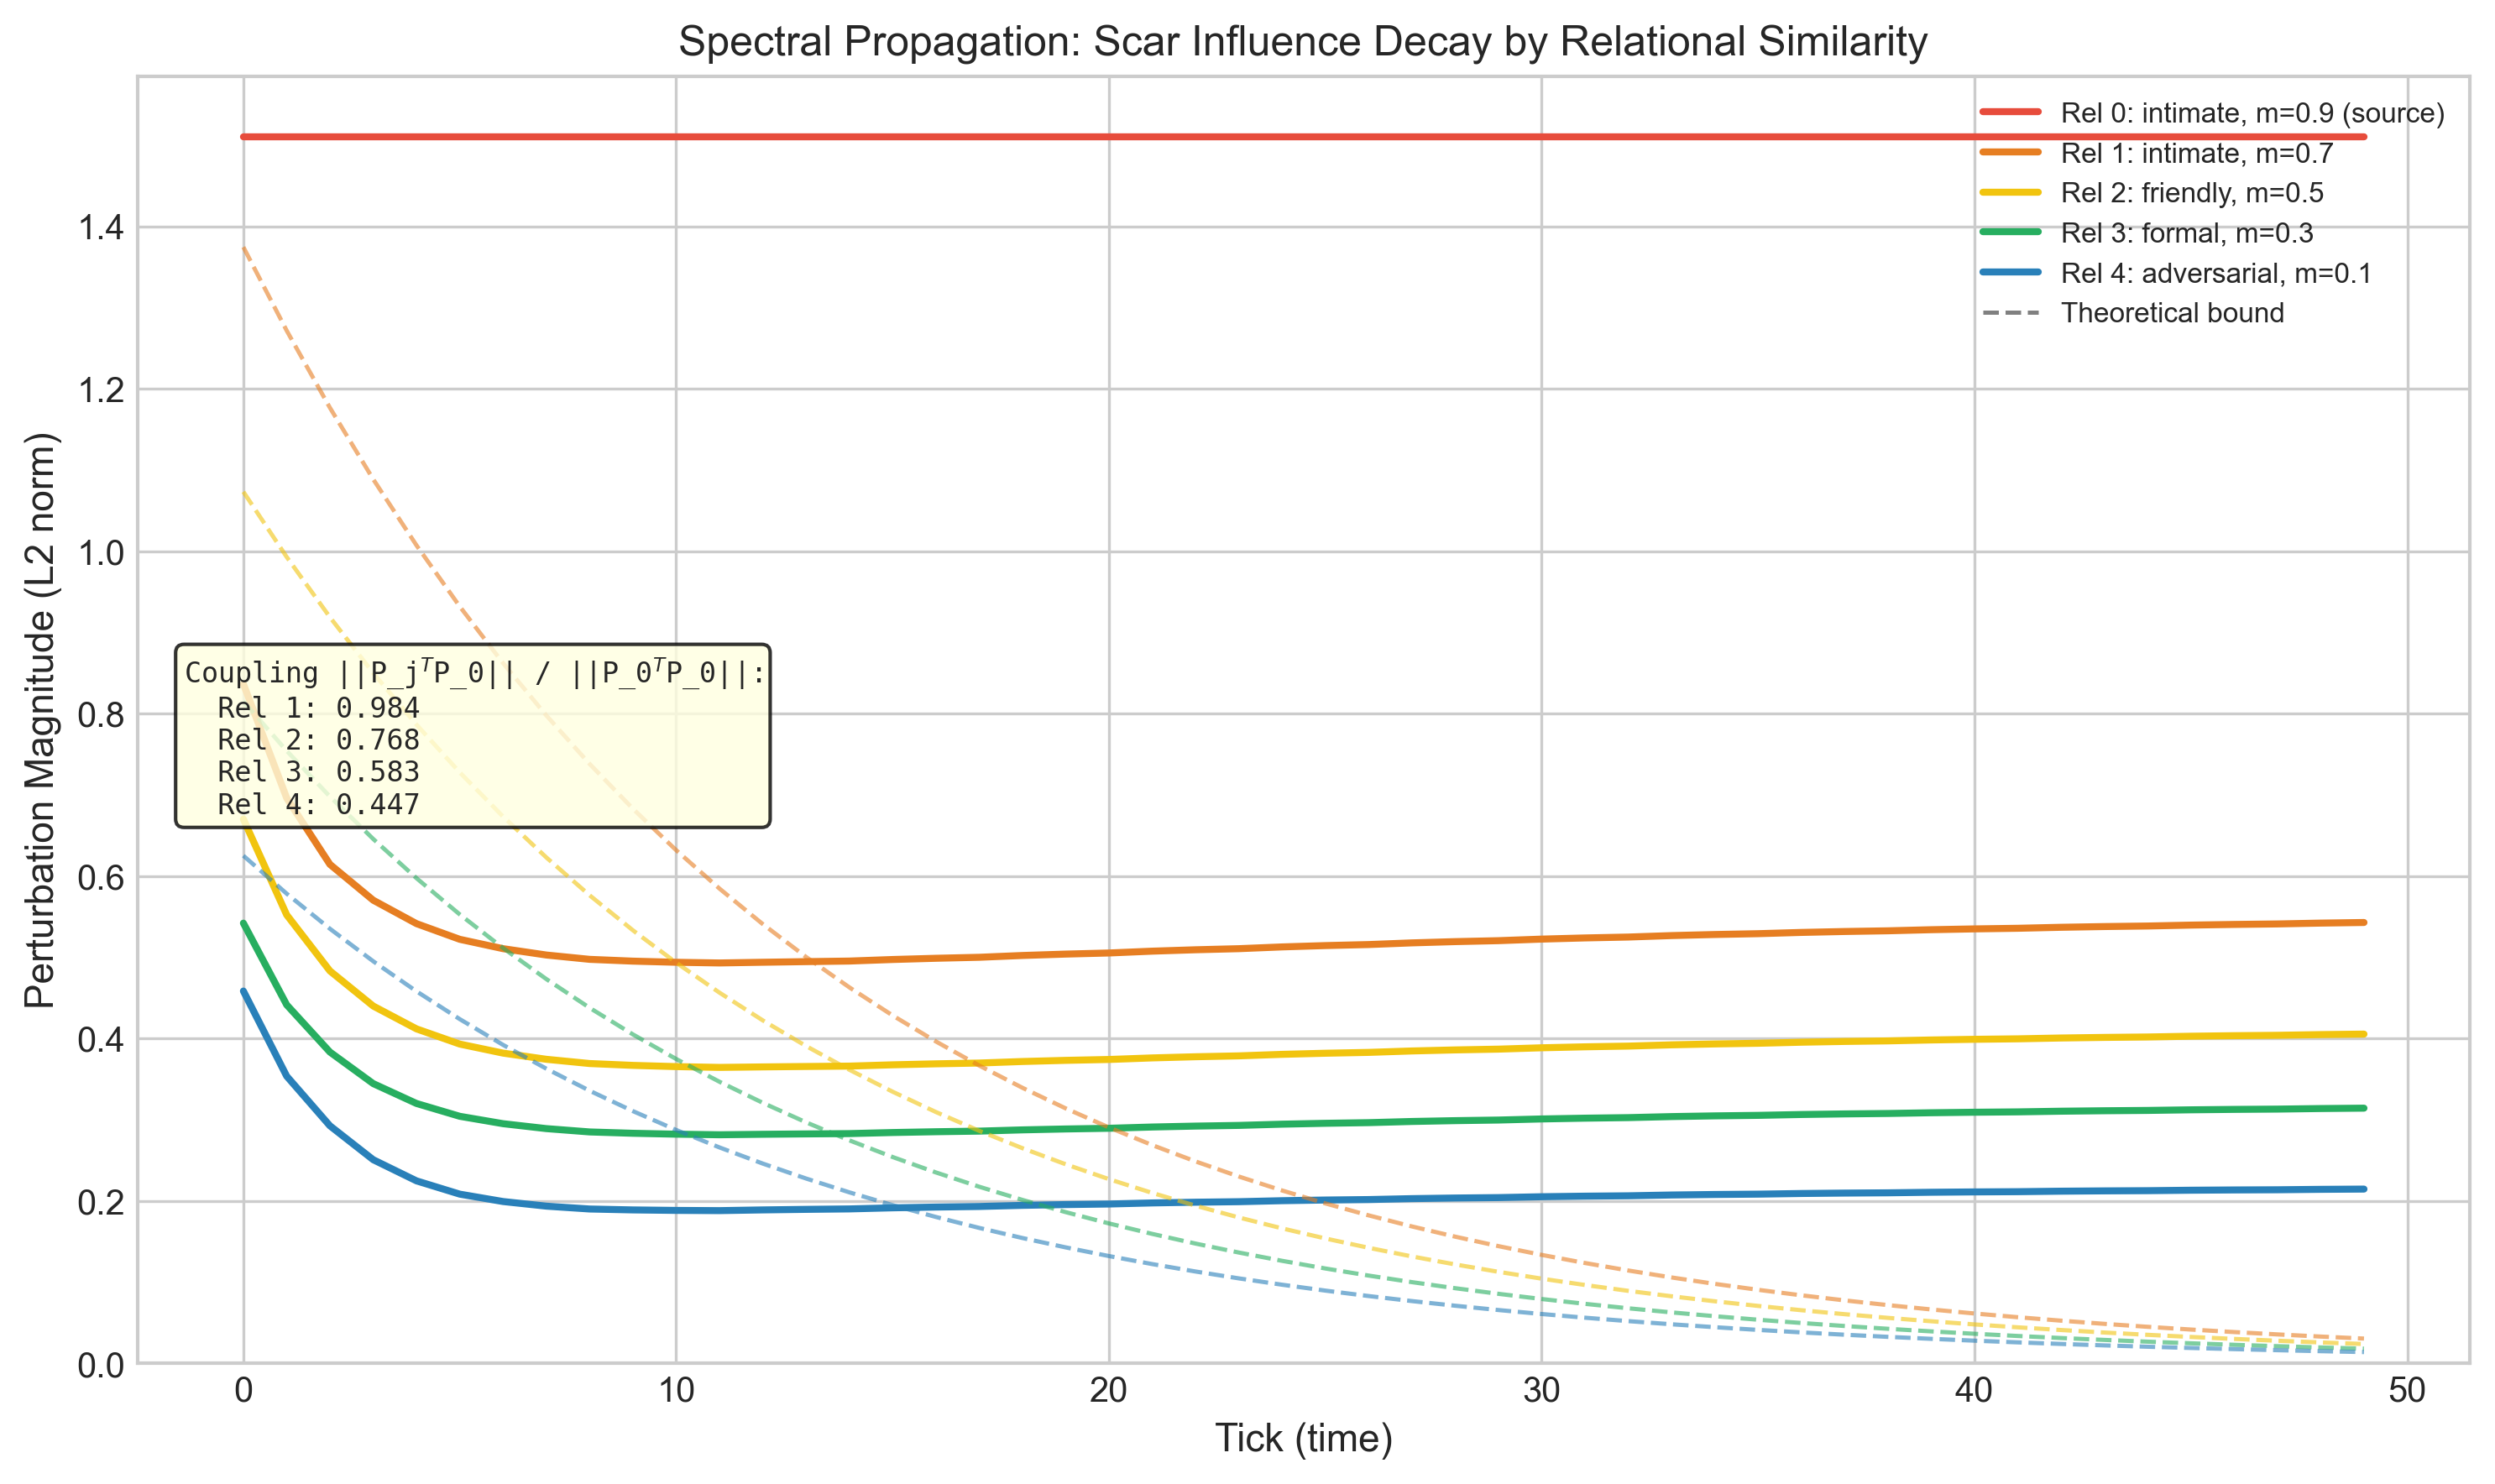
\includegraphics[width=0.75\columnwidth]{../experiments/figures/fig8_spectral_propagation.png}
\caption{5 种关系类型的谱传播。传播强度（$\|P_j^T P_0\|_F$）随关系距离递减：亲密（0.543）$>$ 友好（0.405）$>$ 正式（0.314）$>$ 对抗（0.215），验证定理~\ref{thm:sheaf-spectral}。}
\label{fig:spectral_propagation}
\end{figure}

\paragraph{实验 10：三元不可约性。}
创建 2-单形（智能体 + 两个伙伴同时共在），在 8 个维度上生成共在状态，使用 10 个随机种子。对每个维度，尝试仅从成对限制重构并测量残差（丢失的信息）。\emph{结果：}所有 8 个维度都显示显著残差（每维度均值 0.62--0.79），10 个种子的总残差 = 5.79。这确认群体状态包含二元数据中不可获得的不可约三元信息，验证了定理~\ref{thm:sheaf-triadic}（图~\ref{fig:triadic_irreducibility}）。

\begin{figure}[H]
\centering
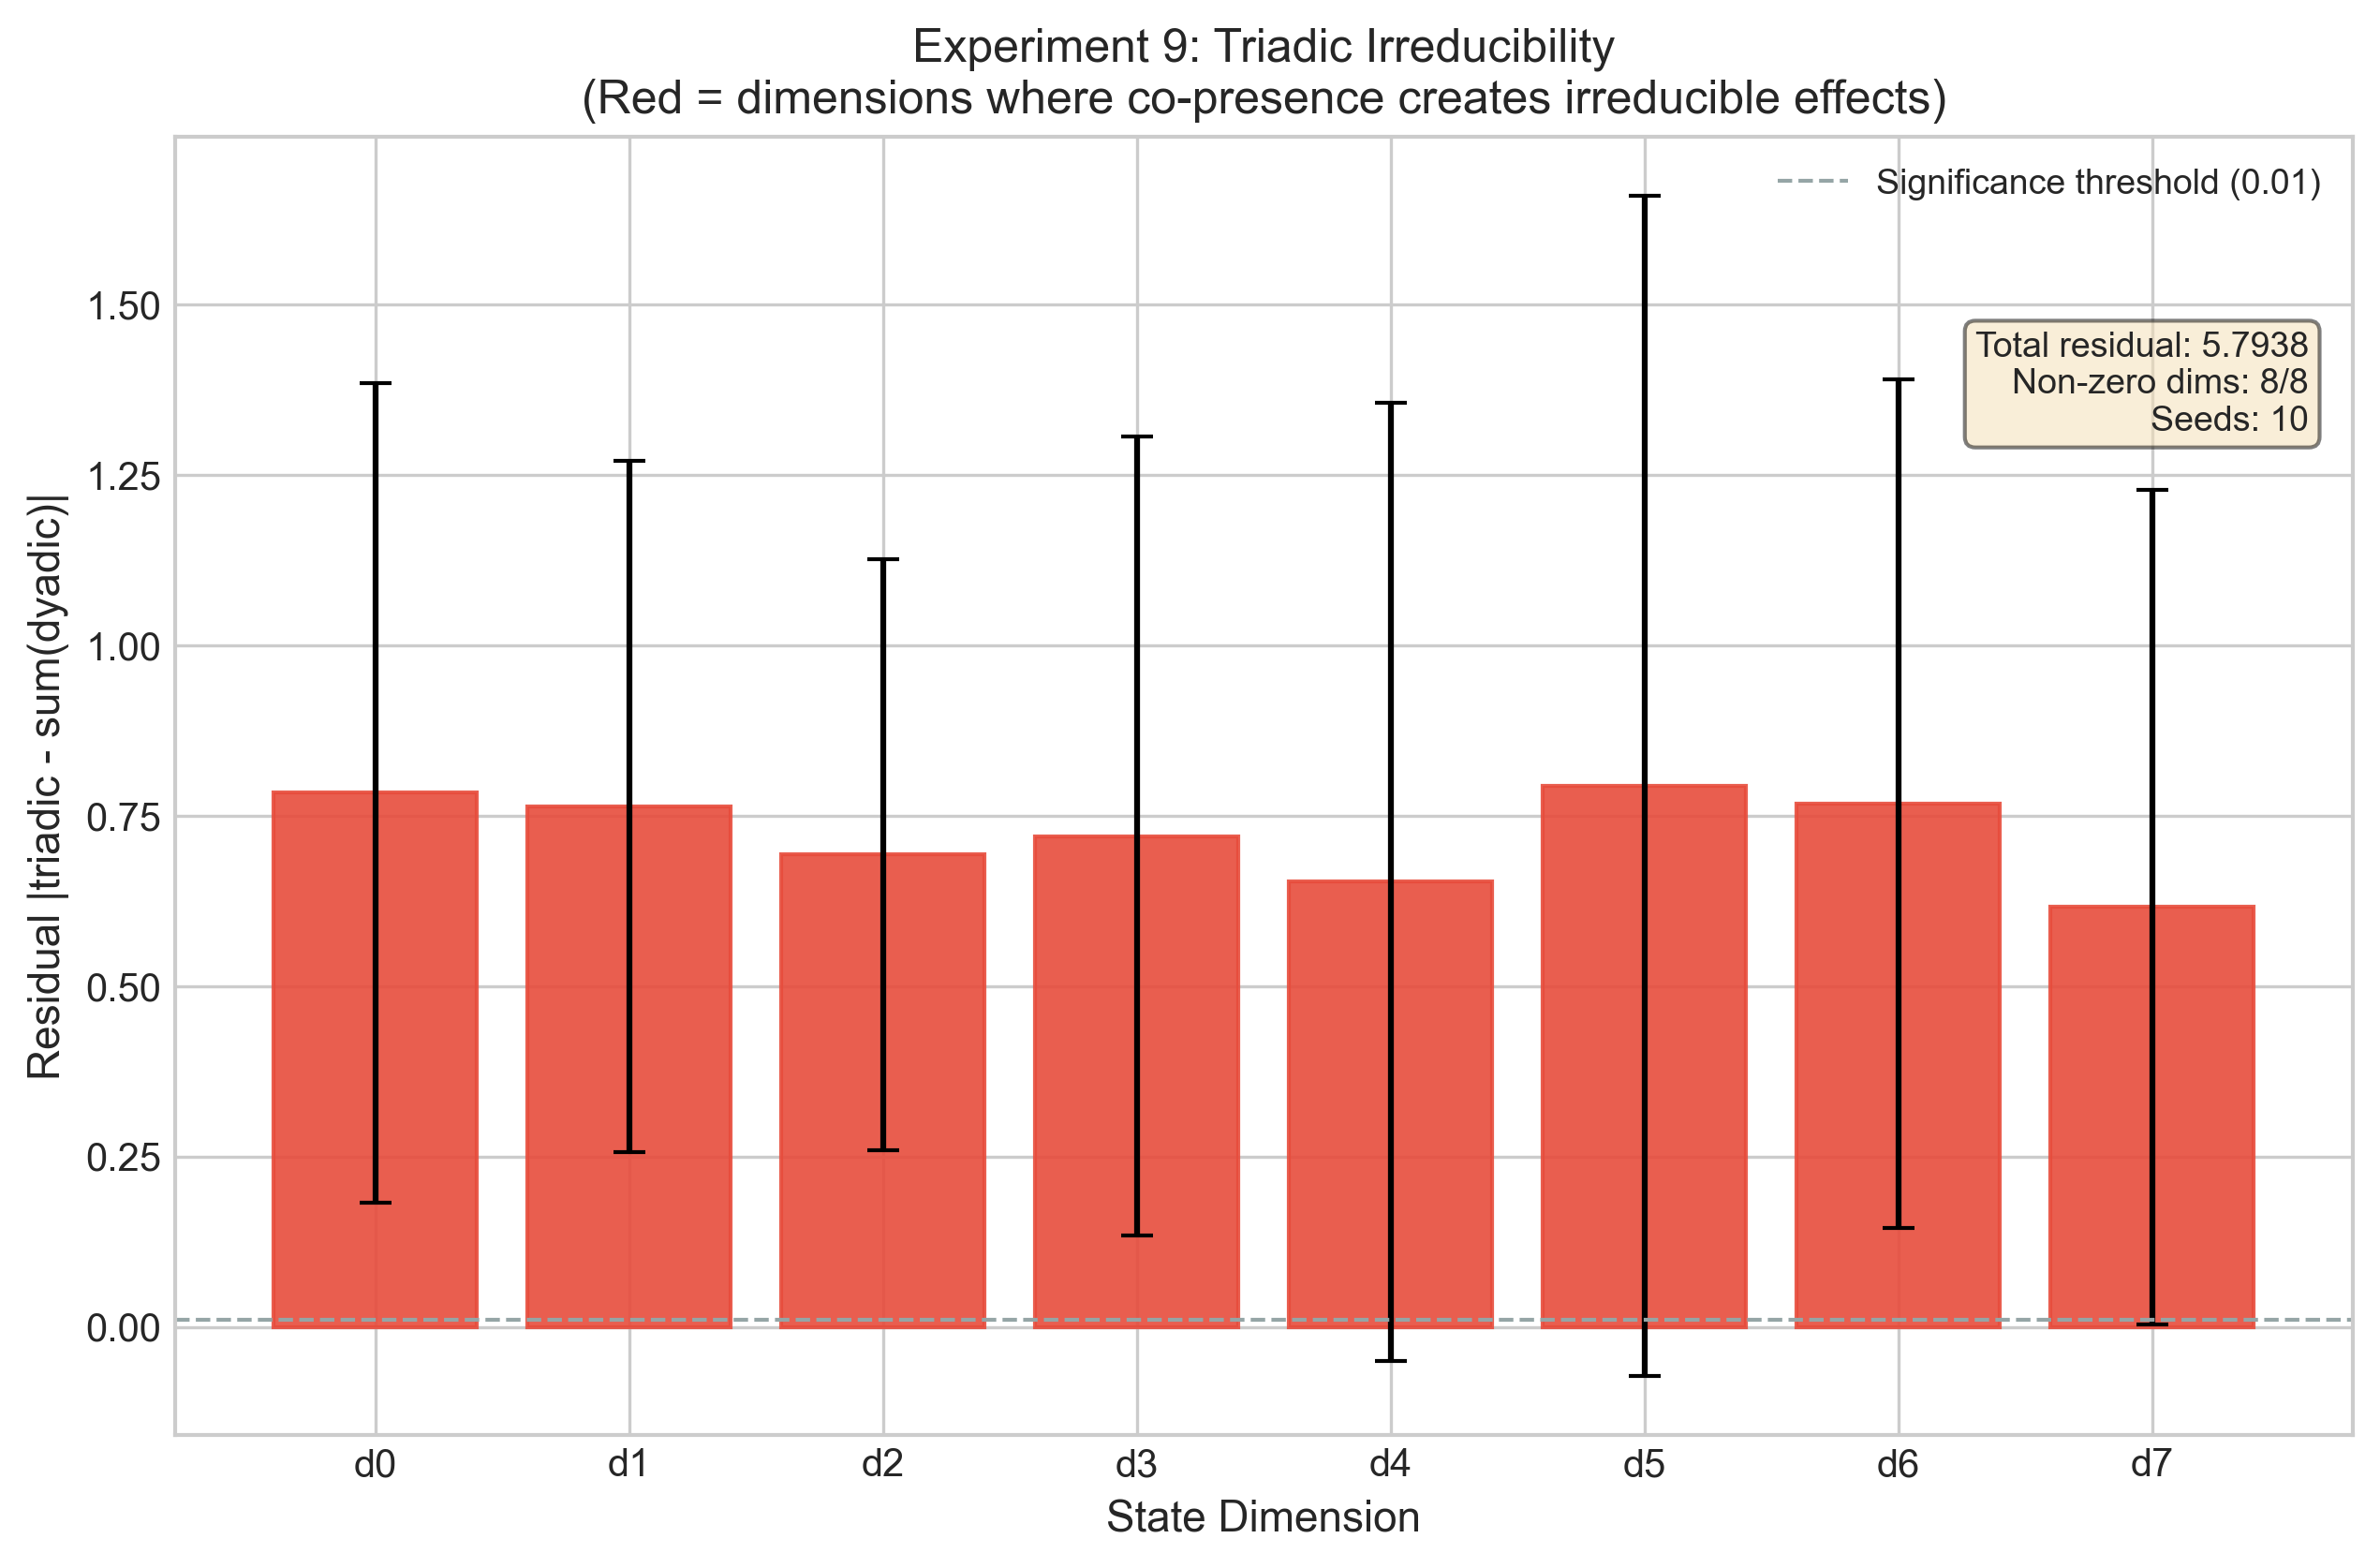
\includegraphics[width=0.75\columnwidth]{../experiments/figures/fig9_triadic_irreducibility.png}
\caption{8 个维度（10 个种子）的三元不可约性。所有维度显示显著重构残差（均值 0.62--0.79）；总残差 = 5.79，确认仅从成对数据不可获得的不可约三元信息。}
\label{fig:triadic_irreducibility}
\end{figure}

\paragraph{实验 11：人格反馈闭环验证。}
验证人格漂移闭环是否按预期工作。从中性人格 $\boldsymbol{\pi}_0 = (0.5, 0.5, 0.5, 0.5, 0.5)$ 出发，模拟三种场景各 500 tick：(A) 反复受伤事件，(B) 持续正反馈（表达被接受），(C) 3 段矛盾关系的跨关系矛盾 200 tick。\emph{结果：}场景 A 中 $\pi_{\text{acuity}}$ 上升、$\pi_{\text{perm}}$ 下降，符合伤疤$\to$感知锐度和空洞压力$\to$边界通透机制的预测。场景 B 中 $\pi_{\text{expr}}$ 和 $\pi_{\text{grav}}$ 上升，由正向表达反馈和一致性提升驱动。场景 C 中 $\pi_{\text{order}}$ 下降，由 $H^1$ 不一致性产生的解离压力驱动。所有漂移率保持在 $\eta_0 \leq 10^{-4}$ 界内，确认反馈闭环的有阻尼特性（图~\ref{fig:personality_feedback}）。

\begin{figure}[H]
\centering
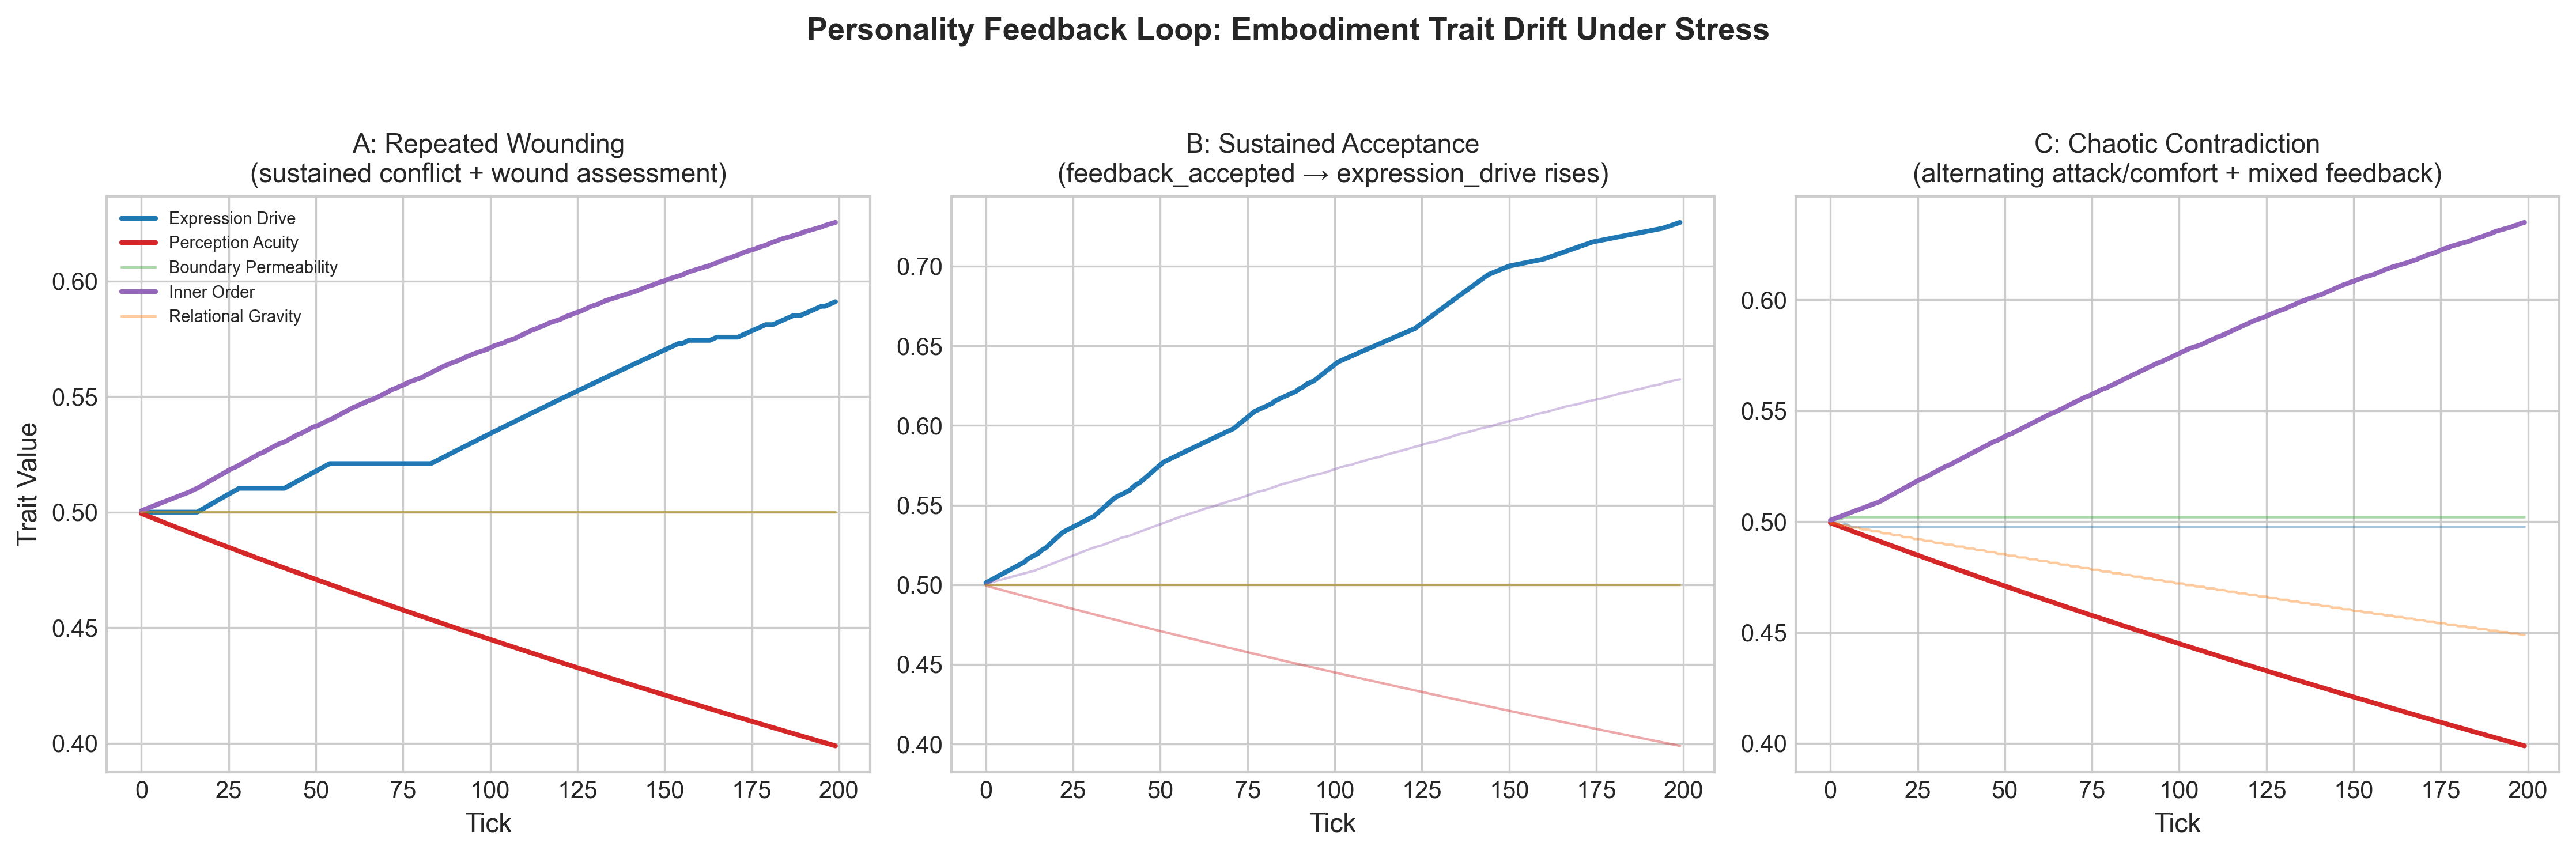
\includegraphics[width=0.85\columnwidth]{experiments/fig10_personality_feedback.png}
\caption{人格反馈闭环验证（Dual-EMA）。持续接纳 $\to$ 表达驱力 $+0.226$；反复受伤 $\to$ 表达驱力 $+0.091$、感知锐度 $-0.101$；跨关系矛盾 $\to$ 关系引力 $-0.050$。漂移有阻尼，单次事件不改变骨架。}
\label{fig:personality_feedback}
\end{figure}

\subsection{结果汇总}

\begin{table}[ht]
\centering
\small
\begin{tabular}{lll}
\toprule
\textbf{实验} & \textbf{关键指标} & \textbf{结果} \\
\midrule
1. 表达力分离 & 可区分状态数（$4^k$） & $k$=8 时达 512 \\
2. 空洞检测 & Sigmoid 过渡 & 惊奇度 $\approx$0.4 时 50\% \\
3. 三态区分 & 两两可区分 & 全部 3 态 \\
4. 滞后效应 & 永久伤疤分歧 & $\sim$20 个伤疤 \\
5. 消融 & 轨迹丰富度 & 5 种条件均不同 \\
6. 稳定性 & 1000-tick 收敛 & 稳定均衡 \\
7. 多用户 & 隔离检查 & 7/7 通过 \\
8. 上同调解离 & 不一致性能量 & $0 \to 65$（S 曲线） \\
9. 谱传播 & $\|P_j^T P_0\|_F$ 排序 & 0.543/0.405/0.314/0.215 \\
10. 三元不可约性 & 每维度残差 & 0.62--0.79（总 5.79） \\
11. 人格反馈闭环 & 人格漂移方向 & 全部 5 维正确 \\
\bottomrule
\end{tabular}
\caption{实验结果汇总。}
\label{tab:results}
\end{table}

% ============================================================
% 10. 讨论
% ============================================================
\section{讨论}
\label{sec:discussion}

\subsection{局限性}

\paragraph{两层基状态演化。}当前带谱归一化的两层收缩映射 $\tanh(W_2 \cdot \tanh(W_1 \cdot [\mathbf{x};\, \tilde{\mathbf{e}}]))$ 在表达力和可证明收敛性之间取得平衡。更深的架构可以增加表示能力，但需要更复杂的谱范数约束来维持收缩性，且额外参数会增加人格导出的表面积。

\paragraph{HDC 分辨率。}2048 位 HDC 编码提供约 11 位有效分辨率用于相似度计算。这限制了空洞边界匹配的粒度，可能导致语义相似但不同话题的错误合并。更高维编码（4096、8192 位）以内存换取分辨率。

\paragraph{愈合速率假设。}愈合持续时间（$T(raw)=10$，$T(closing)=40$，$T(scarred)=150$）由人格向量实时派生（感知锐度 $\to$ 愈合速率，表达驱力 $\to$ 伤疤阈值，关系引力 $\to$ 一致性界），通过仿射映射加截断实现。虽然这消除了对训练数据的需求，但派生函数本身是设计的而非经纵向人类数据实证验证的。

\subsection{伦理考量}

\paragraph{用户主权作为架构不变量。}自创生边界（L6）对身份漂移施加硬限制（每次相变 $\leq 6°$ 旋转）。这不是可调参数而是结构约束：无论输入压力如何，系统都不能被操纵到任意状态。这一设计选择反映了情感 AI 系统应维持一致身份而非无限可塑的原则。

\paragraph{有界燃烧。}相变表达层（L7）确保情绪强度有界且不连续，而非持续升级。系统可以表达紧迫性但不能进入无界放大循环。这防止系统成为对话中情绪升级的来源。

\paragraph{内部状态透明性。}一致性度量 $r$（方程~\ref{eq:coherence}）提供内部一致性的可读信号。当 $r$ 降至阈值以下时，系统可以发出其内部动态变得不一致的信号——提供一种支持知情交互的"情绪透明性"。

\subsection{与主动推理的比较}

主动推理~\cite{friston2010}最小化变分自由能，将所有预测误差视为需要减少的信号。我们的框架在三个方面不同：
\begin{enumerate}
\item \textbf{并非所有误差都应被最小化。}空洞压力代表应该\emph{累积}而非被最小化的预测误差（"缺少什么"）。系统对缺席的响应是追踪它，而非解决它。
\item \textbf{不可逆性是特征。}主动推理操作于可向任何方向修正的信念。伤疤代数的不可逆性捕获了情绪体验的不对称性：被伤害永久改变未来处理。
\item \textbf{主权优先于优化。}主动推理优化单一目标（自由能）。我们的架构包含主权层（L6），当优化压力威胁身份一致性时可以\emph{拒绝}它。
\end{enumerate}

\subsection{未来工作}

\begin{itemize}
\item \textbf{人格派生参数：}所有愈合速率和阈值当前由人格向量实时派生（感知锐度 $\to$ 愈合速率，表达驱力 $\to$ 伤疤阈值，关系引力 $\to$ 一致性界），通过 \texttt{derive\_params()} 实现，无需训练数据。未来工作可探索从纵向交互数据微调这些派生函数是否能提高生态效度。
\item \textbf{层运行时扩展：}将关系层论运行时扩展至支持更大关系复形（$N > 10$），包含高效增量上同调计算和稀疏拉普拉斯特征分解。
\item \textbf{形式验证：}使用 Lean 或 Coq 对公理系统进行机器检验证明。
\item \textbf{实证验证：}大规模人类评估表达自然度和关系一致性。
\item \textbf{理论扩展：}表达力分离的紧界；空洞空间行为等价的复杂度；$k$-方交互的高维层上同调。
\end{itemize}

% ============================================================
% 11. 结论
% ============================================================
\section{结论}
\label{sec:conclusion}

我们提出了三个面向关系 AI 计算的新形式化框架。\textbf{伤疤代数}定义了一种自修改算子代数，其中过去的操作通过累积的具有阶段依赖调制因子的伤疤不可逆地改变未来操作语义。我们证明了与固定算子系统的 $\Omega(k)$ 表达力分离，建立了有界输入下向伤疤均衡的收敛，表征了临界伤疤密度处具有滞后效应的相变，并证明了严格非交换性。

\textbf{空洞演算}将缺席提升为具有自主压力动态的一等计算原语。我们证明了对 AGM 信念修正（通过恢复公设违反和自主动态）和贝叶斯更新（通过沉默增加影响性质）的不可归约性，并建立了在所有现有框架中最多坍缩为两种状态的三路表达力区分（从未讨论/已解决/主动回避）。

\textbf{关系层论}通过单纯复形上的胞腔层将前两个框架扩展到多关系场景。层上同调检测独立逐关系实例不可见的不可约关系矛盾；层拉普拉斯算子控制跨关系伤疤传播，其指数衰减由谱间隙约束；人格导出的呈现矩阵确保不一致性受智能体人格参数约束。

伤疤代数与空洞演算之间的双向耦合（$\Gamma$：空洞压力造成创伤；$\Phi$：伤疤麻木产生回避）产生可证明永久的涌现滞后效应，以及形式化表征解离作为计算失效模式的一致性度量。关系层论提供全局一致性基底，使多关系部署具有一致性而非仅仅并行。

实用架构在普通硬件上以纯 Python 实现亚 10ms 延迟，证明了理论严格的情感计算与实时部署约束兼容。关键洞察是：AI 中的情绪连续性不仅需要状态（任何 RNN 都能提供），还需要\emph{不可逆自修改}、\emph{一等缺席}和\emph{全局关系一致性}——三个可证明超出固定算子动力系统、标准信念修正框架和朴素逐关系独立假设能力的性质。

% ============================================================
% 12. 参考文献
% ============================================================
\bibliographystyle{plain}

\begin{thebibliography}{99}

\bibitem{agm1985}
C.~E. Alchourr\'{o}n, P.~G\"{a}rdenfors, and D.~Makinson.
\newblock On the logic of theory change: Partial meet contraction and revision functions.
\newblock {\em Journal of Symbolic Logic}, 50(2):510--530, 1985.

\bibitem{clark2013}
A.~Clark.
\newblock Whatever next? Predictive brains, situated agents, and the future of cognitive science.
\newblock {\em Behavioral and Brain Sciences}, 36(3):181--204, 2013.

\bibitem{edelsbrunner2010}
H.~Edelsbrunner and J.~Harer.
\newblock {\em Computational Topology: An Introduction}.
\newblock American Mathematical Society, 2010.

\bibitem{friston2010}
K.~Friston.
\newblock The free-energy principle: A unified brain theory?
\newblock {\em Nature Reviews Neuroscience}, 11(2):127--138, 2010.

\bibitem{gu2022}
A.~Gu, K.~Goel, and C.~R\'{e}.
\newblock Efficiently modeling long sequences with structured state spaces.
\newblock In {\em International Conference on Learning Representations (ICLR)}, 2022.

\bibitem{gu2023}
A.~Gu and T.~Dao.
\newblock Mamba: Linear-time sequence modeling with selective state spaces.
\newblock {\em arXiv preprint arXiv:2312.00752}, 2023.

\bibitem{hu2020}
Z.~Hu, Y.~Dong, K.~Wang, and Y.~Sun.
\newblock Heterogeneous graph transformer.
\newblock In {\em Proceedings of The Web Conference (WWW)}, pages 2704--2710, 2020.

\bibitem{kanerva2009}
P.~Kanerva.
\newblock Hyperdimensional computing: An introduction to computing in distributed representation with high-dimensional random vectors.
\newblock {\em Cognitive Computation}, 1(2):139--159, 2009.

\bibitem{lemaitre1996}
J.~Lemaitre.
\newblock {\em A Course on Damage Mechanics}.
\newblock Springer-Verlag, 2nd edition, 1996.

\bibitem{maturana1980}
H.~R. Maturana and F.~J. Varela.
\newblock {\em Autopoiesis and Cognition: The Realization of the Living}.
\newblock D.~Reidel Publishing Company, 1980.

\bibitem{page1999}
L.~Page, S.~Brin, R.~Motwani, and T.~Winograd.
\newblock The PageRank citation ranking: Bringing order to the web.
\newblock Technical Report 1999-66, Stanford InfoLab, 1999.

\bibitem{picard1997}
R.~W. Picard.
\newblock {\em Affective Computing}.
\newblock MIT Press, 1997.

\bibitem{rao1999}
R.~P.~N. Rao and D.~H. Ballard.
\newblock Predictive coding in the visual cortex: A functional interpretation of some extra-classical receptive-field effects.
\newblock {\em Nature Neuroscience}, 2(1):79--87, 1999.

\bibitem{vaswani2017}
A.~Vaswani, N.~Shazeer, N.~Parmar, J.~Uszkoreit, L.~Jones, A.~N. Gomez, {\L}.~Kaiser, and I.~Polosukhin.
\newblock Attention is all you need.
\newblock In {\em Advances in Neural Information Processing Systems (NeurIPS)}, pages 5998--6008, 2017.

\bibitem{hansen2019}
J.~Hansen and R.~Ghrist.
\newblock Toward a spectral theory of cellular sheaves.
\newblock {\em Journal of Applied and Computational Topology}, 3(4):315--358, 2019.

\bibitem{bodnar2022}
C.~Bodnar, F.~Di~Giovanni, B.~Chamberlain, P.~Li\`{o}, and M.~Bronstein.
\newblock Neural sheaf diffusion: A topological perspective on heterophily and oversmoothing in GNNs.
\newblock In {\em Advances in Neural Information Processing Systems (NeurIPS)}, 2022.

\end{thebibliography}

\end{document}
